\PassOptionsToPackage{quiet}{fontspec}
\documentclass[12pt,a4paper,UTF8]{article}
\usepackage{thesis} % 格式控制
\usepackage{indentfirst}
\usepackage{amsmath} % 数学公式支持
\usepackage{amsfonts} % 数学字体支持
\usepackage{amssymb} % 数学符号支持
\usepackage{graphicx} % 图片插入支持
\usepackage{float} % 浮动体位置控制，支持 [H] 选项
\usepackage{caption} % 图表标题格式控制
\usepackage{geometry} % 页面布局控制
\usepackage{setspace} % 行距控制
\usepackage{xeCJK} % 中文字体支持
\usepackage{fontspec} % 字体设置
\usepackage[most]{tcolorbox} % 高亮按键命令
\setlength{\parindent}{2em} % 控制首行缩进  
\addtolength{\parskip}{3pt} % 控制段落距离  
\onehalfspacing % 1.5倍行距  
\graphicspath{{./figures/}} % 指定图片所在文件夹  
\setCJKmainfont{SimSun}
% 定义中文字体命令
\setCJKfamilyfont{hei}{SimHei} 

\classname{天线理论与设计}  % 设置课程名称
\makepagestyle{}{\printclassname ~实验报告}

% 自定义命令
\newtcbox{\keyblue}{on line,
  colframe=blue!60!black, colback=blue!10,
  boxrule=0.8pt, arc=2pt, boxsep=0pt, left=2pt, right=2pt, top=1pt, bottom=1pt,
  tcbox raise base, fontupper=\color{blue}\bfseries}

\begin{document}
\maketitlepage{HFSS半波偶极子天线设计}{玉泉教4-302}{郑智瑄}{3230103913}{\today}{王浩刚} %封面页 

\maketoc    %目录页

\section{实验原理}

本次实验旨在通过 Ansys HFSS 软件仿真架设在有限尺寸方形地平面上的单极天线（Monopole Antenna），分析其输入阻抗（$Z_{in}$）、电压驻波比（VSWR）及三维辐射方向图。实验核心原理基于镜像理论、四分之一波长谐振以及有限地平面效应。

\subsection{镜像理论 (Image Theory)}

镜像理论是分析置于理想电导体（PEC）平面上天线的基本方法。%如Figure~\ref{fig:image_theory}~所示，
长度为 $L$ 的垂直单极天线（图 a）在 PEC 平面上方产生的电磁场，与总长度为 $2L$ 的中心馈电偶极天线（图 b）在上半空间产生的电磁场完全相同。

\begin{figure}[H]
   \centering
   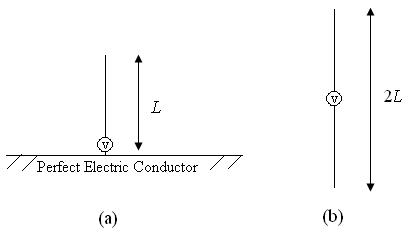
\includegraphics[width=0.7\textwidth]{e1.jpg}
   \caption{镜像理论示意图}
   \label{fig:image_theory}
\end{figure}

根据镜像理论，单极天线具有以下特性：

\begin{itemize}
    \item \textbf{辐射空间：} 仅在 PEC 平面上方的半空间内辐射能量。
    \item \textbf{输入阻抗：} 单极天线的输入阻抗为等效偶极天线的一半，即
    \begin{equation}
        Z_{\text{monopole}} = \frac{1}{2} Z_{\text{dipole}}
    \end{equation}
    \item \textbf{方向性：} 辐射能量集中在半空间，方向性系数是等效偶极天线的两倍。
\end{itemize}

\subsection{四分之一波长谐振原理}

在 $f = 300 \text{ MHz}$ 时，自由空间波长为：
\begin{equation}
    \lambda = \frac{c}{f} = \frac{3 \times 10^8 \text{ m/s}}{300 \times 10^6 \text{ Hz}} = 1 \text{ 米}
\end{equation}

四分之一波长单极天线（$L = \lambda/4 = 0.25 \text{ m}$）等效于半波偶极天线（$2L = \lambda/2$）。理想半波偶极天线谐振阻抗约为 $73 \Omega$，因此理想四分之一波长单极天线的输入阻抗应为：
\begin{equation}
    Z_{in} \approx \frac{1}{2} \times 73 \Omega \approx 36.5 \Omega
\end{equation}

其辐射方向图%如图~\ref{fig:radiation_pattern}~所示，
在水平面呈全向辐射，在垂直面上最大辐射方向沿地平面（仰角 $0^\circ$），天顶方向（仰角 $90^\circ$）辐射为零。

\begin{figure}[H]
   \centering
   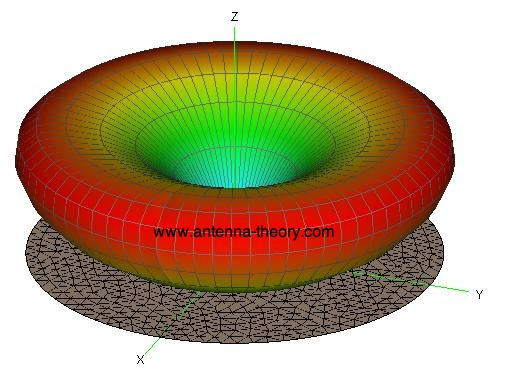
\includegraphics[width=0.6\textwidth]{e2.jpg}
   \caption{四分之一波长单极天线经典辐射方向图}
   \label{fig:radiation_pattern}
\end{figure}

\subsection{有限地平面的影响}

镜像理论基于无限大地平面假设。实际中，有限地平面会引入\textbf{边缘衍射（Edge Diffraction）}效应，使特性偏离理论值：

\begin{itemize}
    \item \textbf{改变输入阻抗：} $Z_{in}$ 将偏离理论值 $36.5 \Omega$。
    \item \textbf{改变辐射方向图：} 在地平面下方产生后瓣，主瓣最大辐射方向可能向上抬起。
\end{itemize}

\section{实验任务}

使用 HFSS 软件模拟一个单极天线，具体要求如下：

\begin{enumerate}
    \item 单极天线的长度设置为 0.25 米；
    \item PEC 接地板是一个 1 米乘 1 米的正方形；
    \item 单极天线需要竖立在接地板的中心上方；
    \item 模拟的频率范围是 200MHz 至 400MHz。
\end{enumerate}

\section{仿真步骤}

\subsection{新建设计工程}

\begin{enumerate}
    \item 运行 \keyblue{Ansys Electronics Desktop Student} 并新建 HFSS 工程，重命名为 monopole；
    
    \item 设置求解类型：在菜单栏中选择 \keyblue{HFSS}-\keyblue{Solution Type}，在弹出窗口中选择 \keyblue{Modal}，完成设置。%：
\end{enumerate}

\begin{figure}[H]
   \centering
   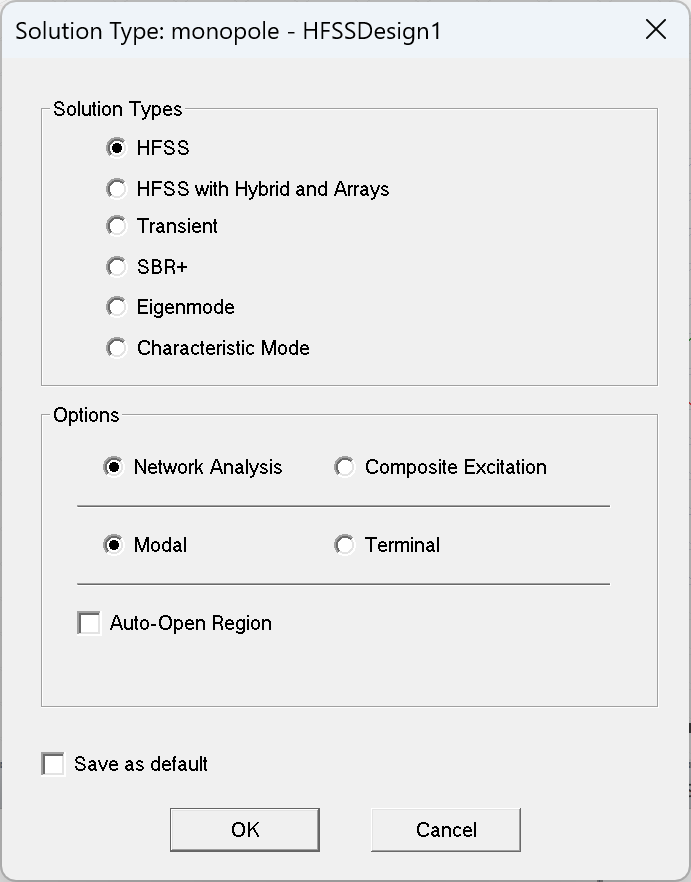
\includegraphics[width=0.6\textwidth]{p1.png}
   \caption{Solution Type 设置}
\end{figure}

\subsection{添加设计变量}

在主菜单栏中选择 \keyblue{HFSS}-\keyblue{Design Properties}，打开设计属性对话框，单击 \keyblue{Add} 按钮，打开 \keyblue{Add Property} 对话框，依次定义变量。%，如下图所示：

\begin{figure}[H]
   \centering
   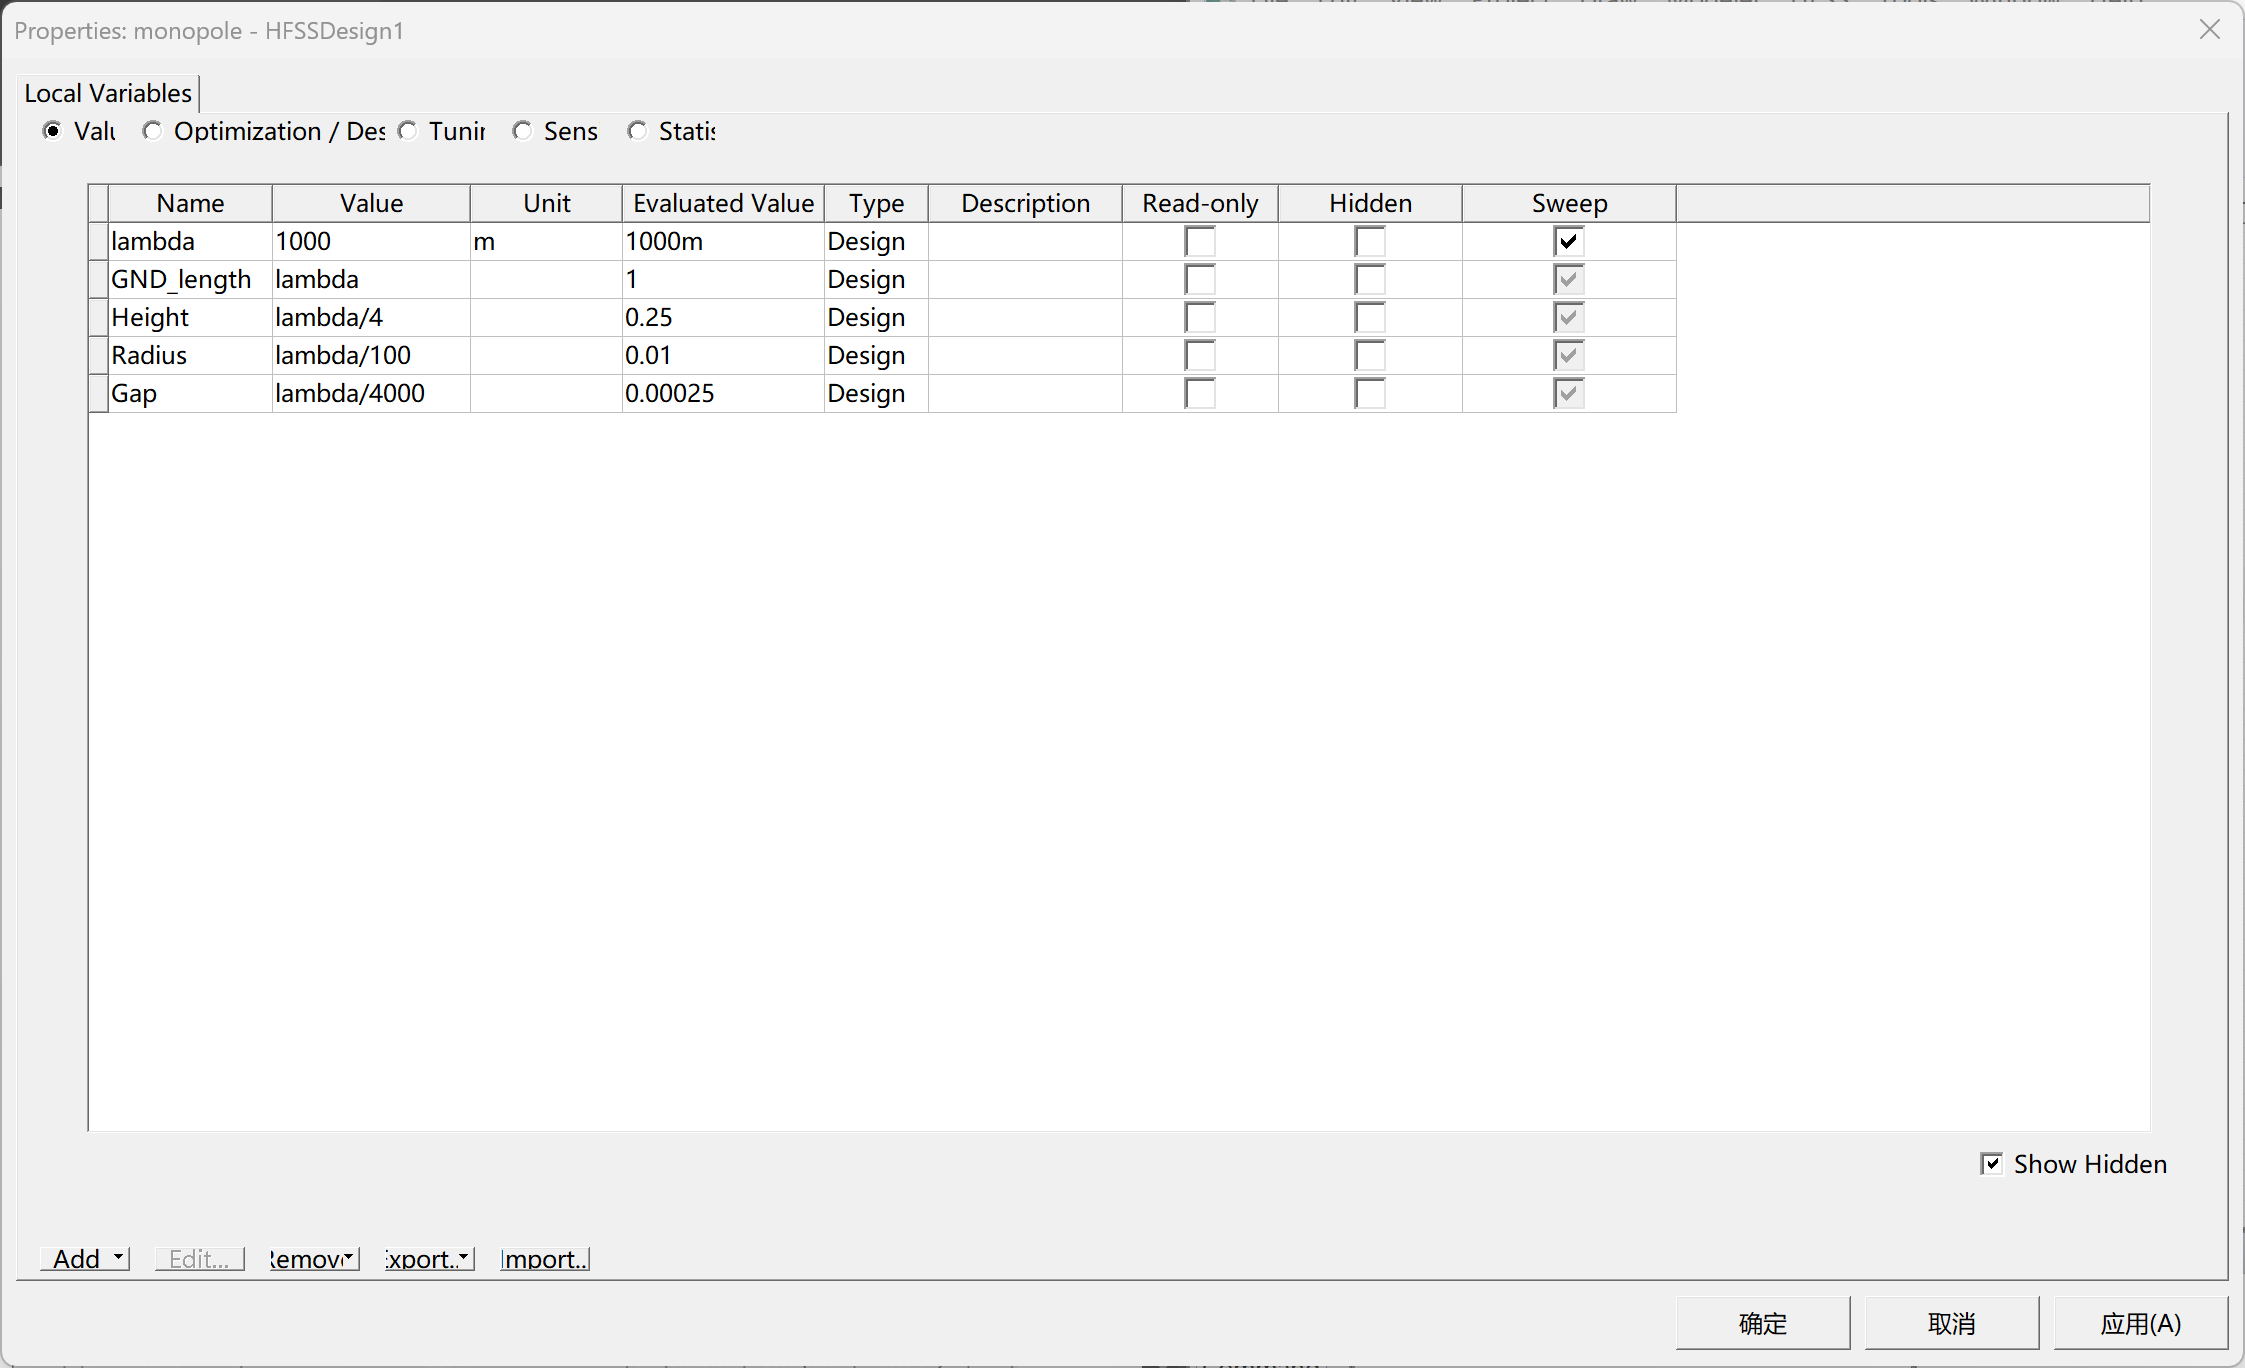
\includegraphics[width=0.8\textwidth]{p2.png}
   \caption{添加设计变量}
\end{figure}

\subsection{天线模型建立}

\subsubsection{创建 GND 矩形面}

\begin{enumerate}
    \item 在主菜单栏中选择 \keyblue{Draw}-\keyblue{Rectangle} 创建矩形面，名称设置为 GND。%：
    
  
    \item 双击操作历史树中的 \keyblue{GND}-\keyblue{CreateRectangle} 节点，打开新建矩形面属性对话框的 Command 选项卡，在选项卡中设置矩形面的中心坐标和边长。%，如下所示：
    
 \begin{figure}[H]
       \centering
       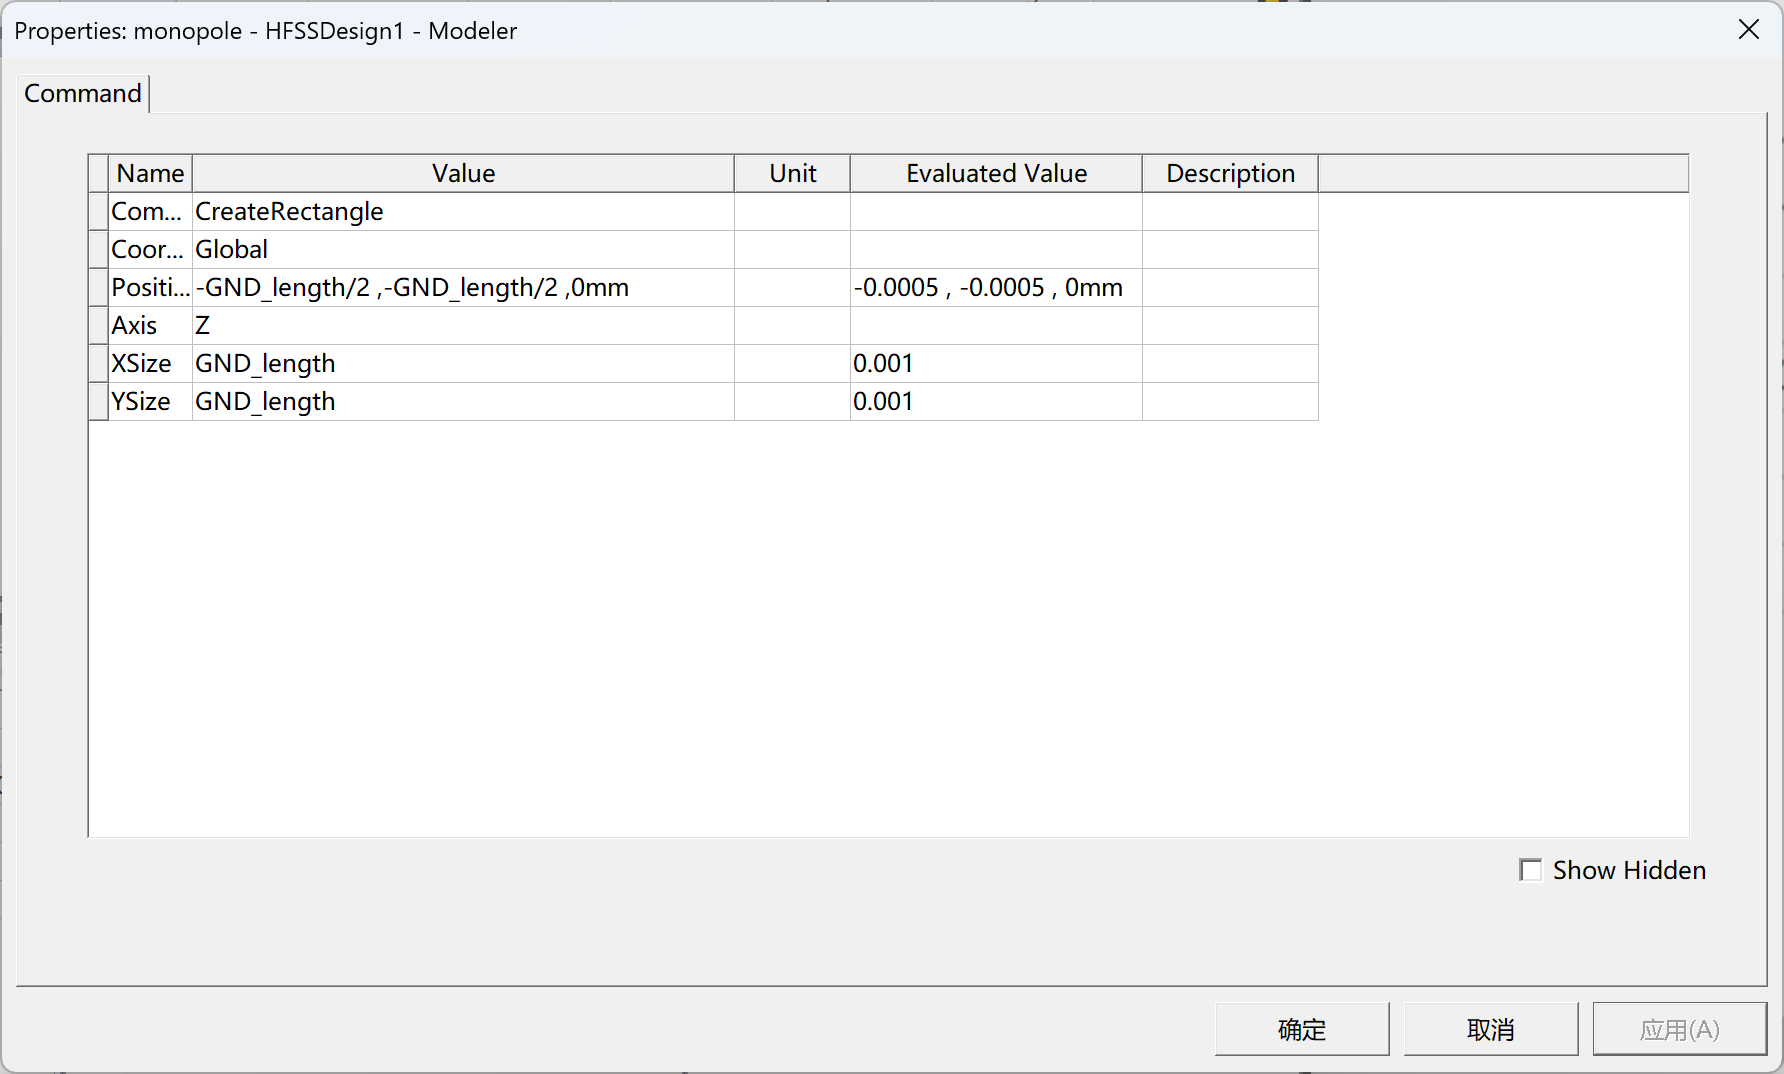
\includegraphics[width=0.8\textwidth]{p4.png}
       \caption{创建 GND 矩形面属性}
   \end{figure}

\end{enumerate}

\subsubsection{生成单极子天线}

\begin{enumerate}
    \item 在主菜单栏中选择 \keyblue{Draw}-\keyblue{Cylinder} 创建圆柱体，圆柱体名称设置为 monopole，材质为 \textit{pec}。%：
    
    \item 双击操作历史树下 \keyblue{monopole}-\keyblue{CreateCylinder} 节点，打开新建圆柱体属性对话框的 Command 选项卡，在选项卡中设置圆柱体的底面圆心坐标、半径和长度。%：
    
   \begin{figure}[H]
       \centering
       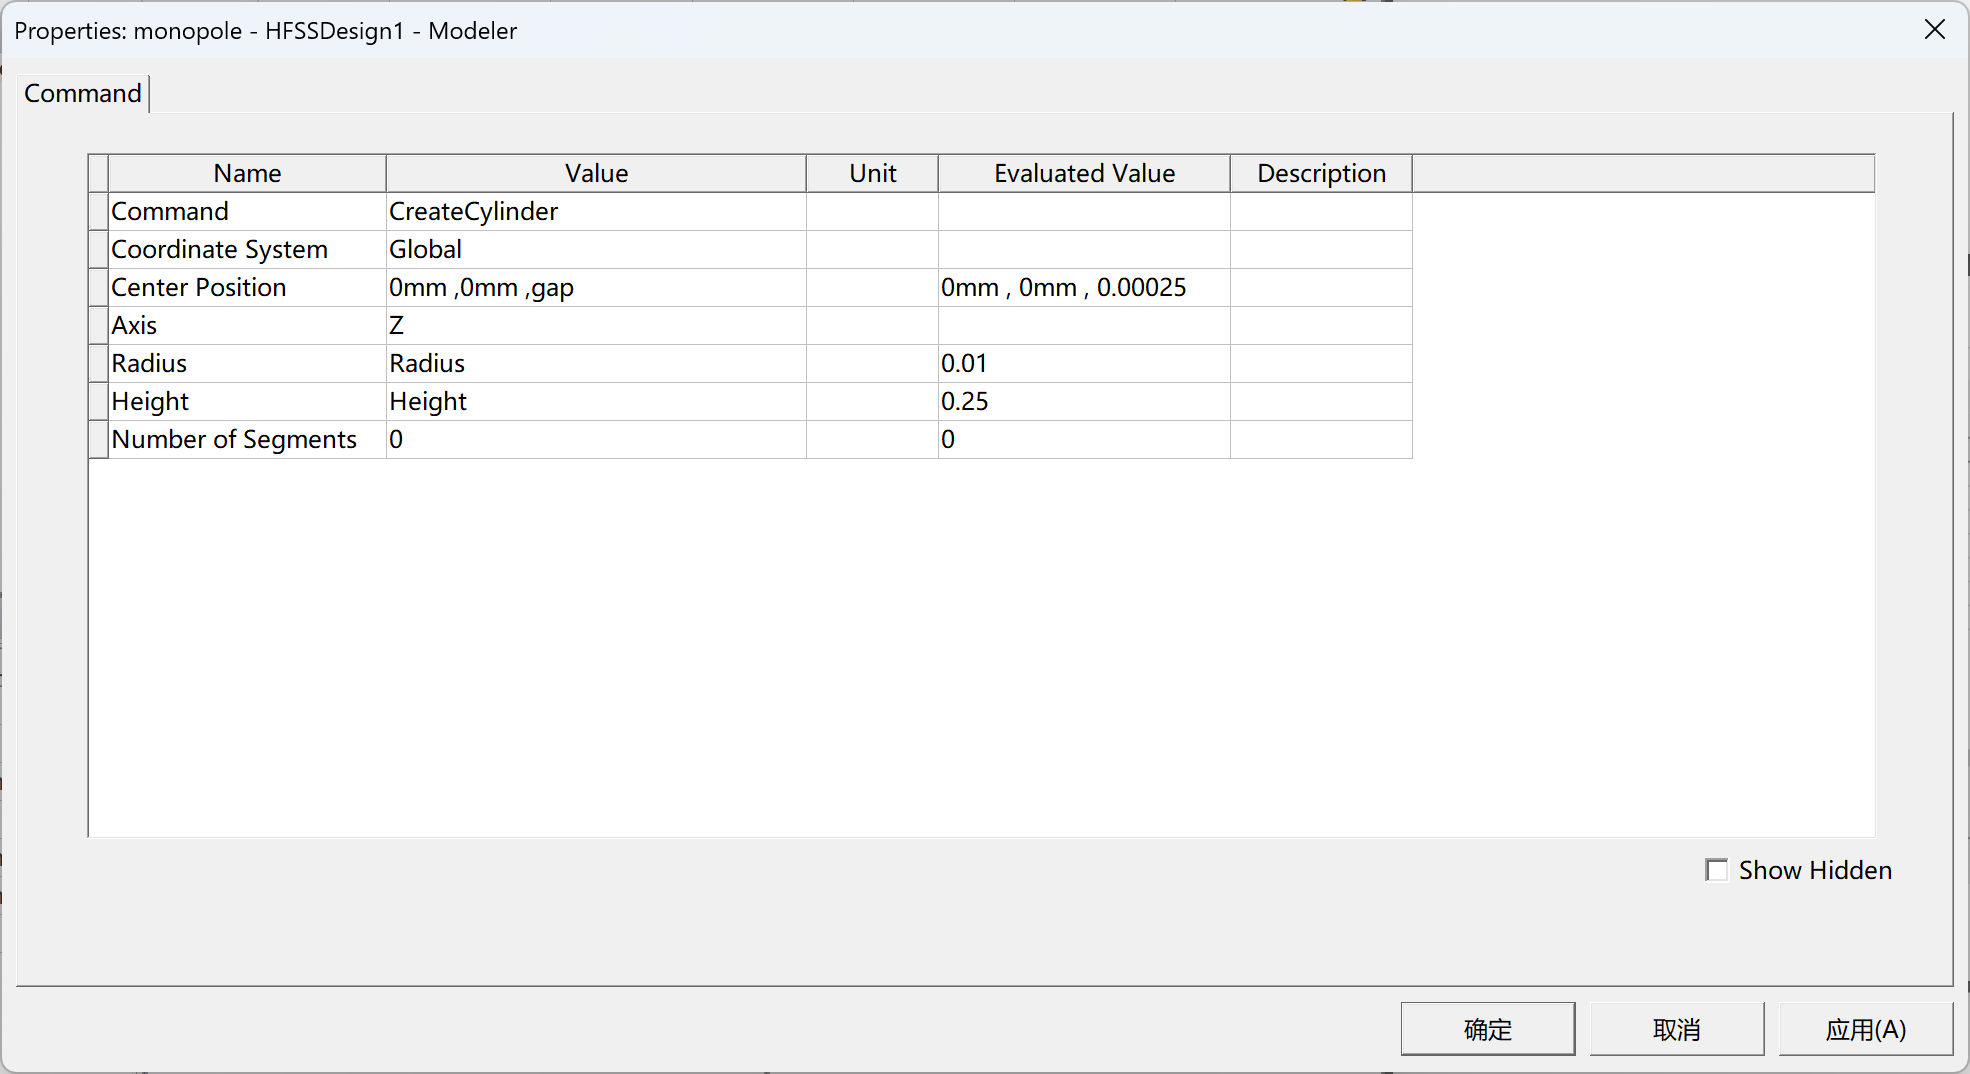
\includegraphics[width=0.8\textwidth]{p6.png}
       \caption{设置单极天线尺寸参数}
   \end{figure}

\end{enumerate}

\subsubsection{设置端口激励}

\begin{enumerate}
    \item 选中 \keyblue{Sheets}-\keyblue{GND}，在弹出的快捷菜单中选中 \keyblue{Assign Boundary}-\keyblue{Perfect E}，并将边界条件名设置为 GND。%，如图所示：
        
    \item 单击工具栏上的 xy 下拉菜单列表框，选择 yz 选项，把当前工作面设置为 yz 平面，然后从主菜单栏中选择 \keyblue{draw}-\keyblue{rectangle}，创建端口矩形；
    
    \item 双击操作历史树中的 \keyblue{sheets}-\keyblue{Rectangle1} 节点，打开新建矩形面属性对话框，把矩形面的名称设置为 \keyblue{Port}；
    
    \item 双击操作历史树下 \keyblue{Port}-\keyblue{CreateRetangle} 节点，在选项卡中设置矩形面的顶点坐标和大小。%：
    
   \begin{figure}[H]
       \centering
       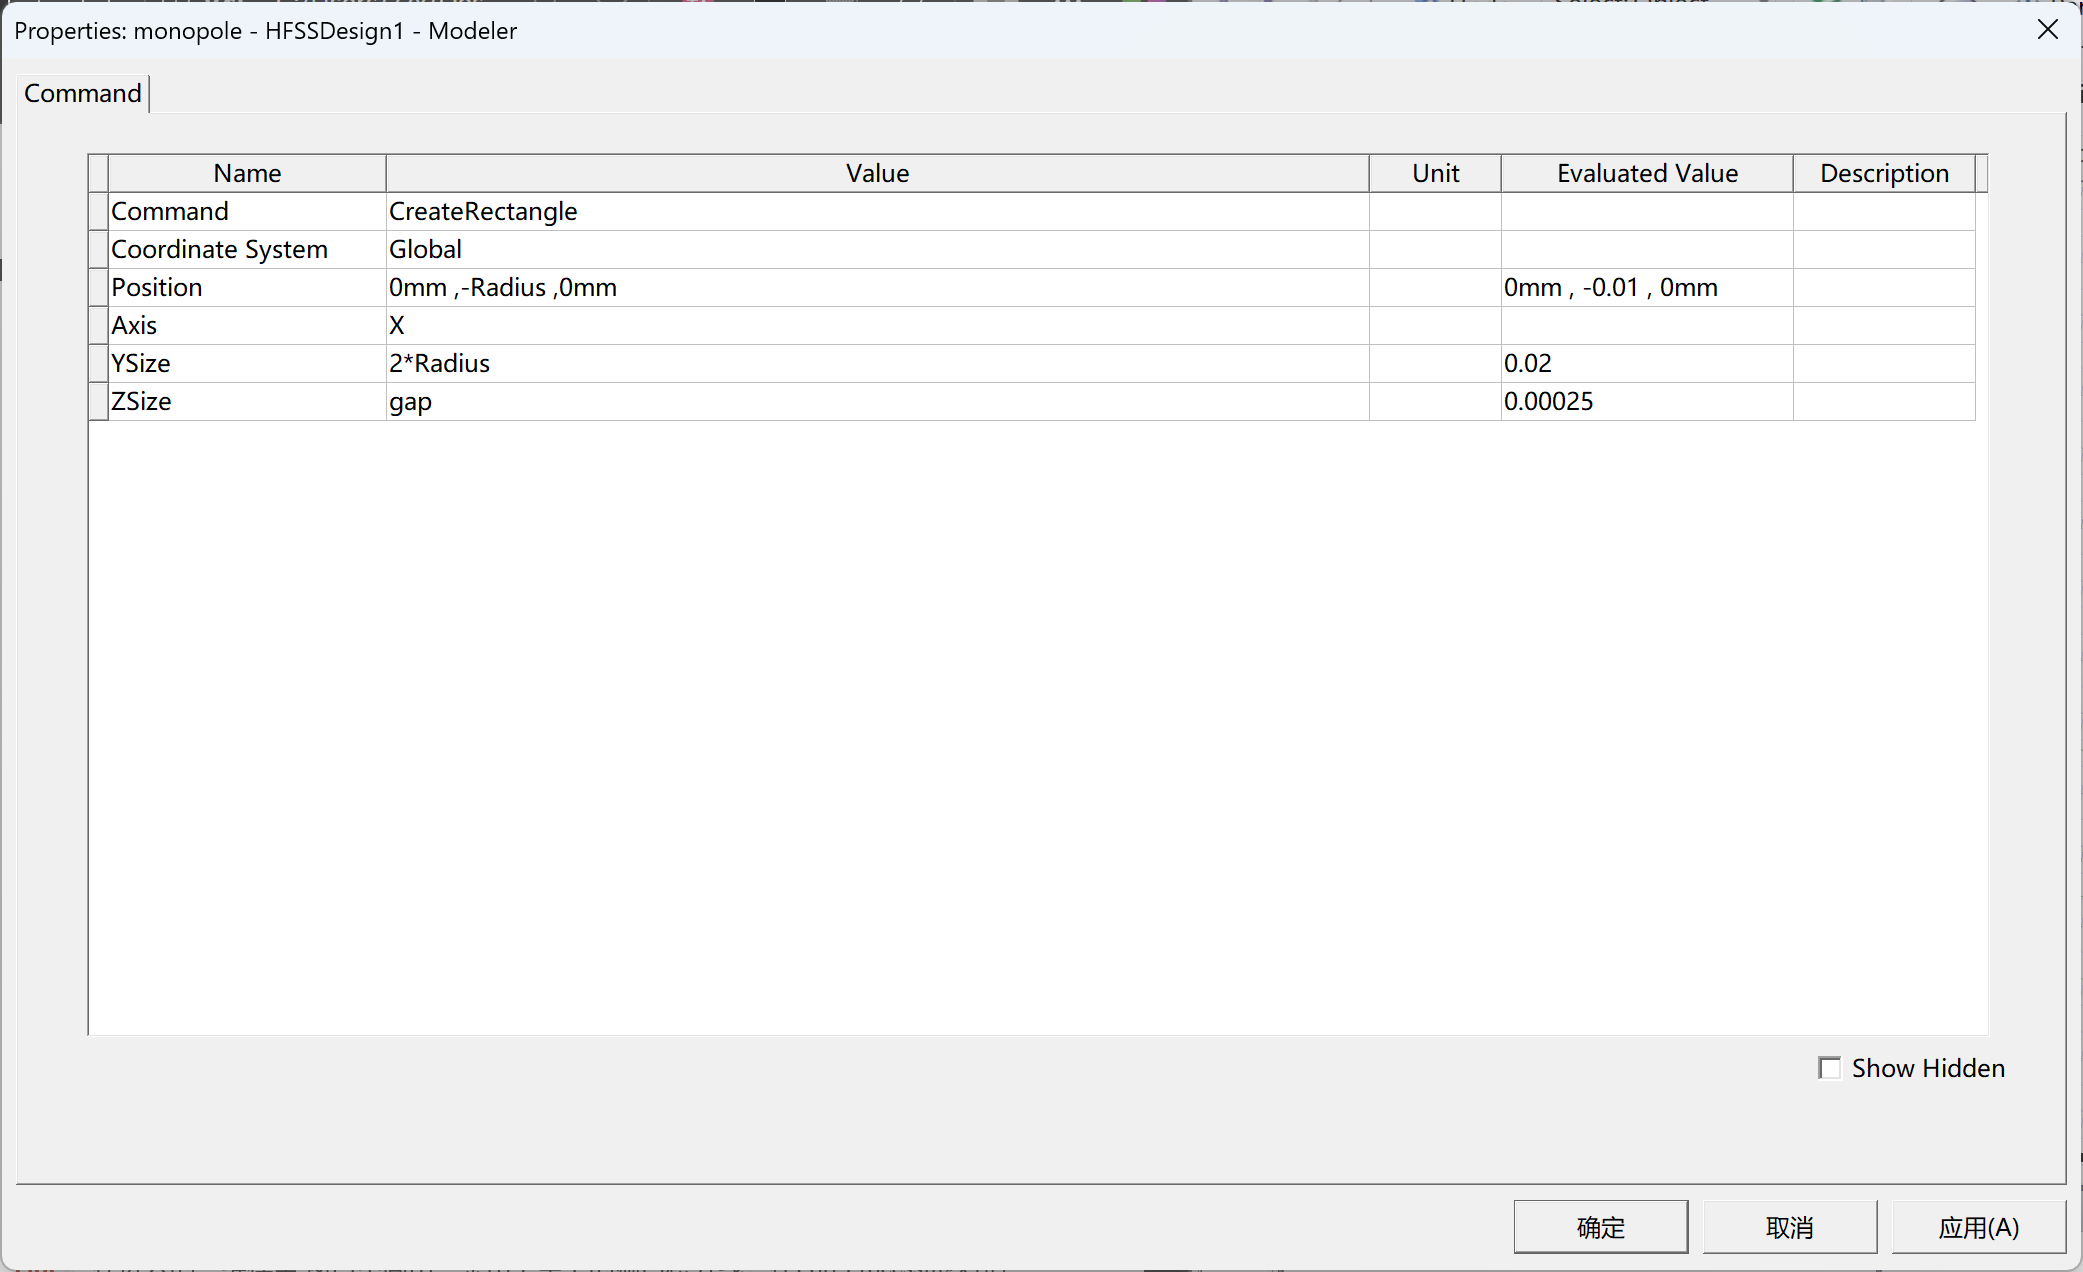
\includegraphics[width=0.8\textwidth]{p11.png}
       \caption{设置端口矩形尺寸}
   \end{figure}
    
    \item 点击操作历史树的 \keyblue{Sheets}-\keyblue{Port}，在菜单中选中 \keyblue{Assign Excitation}-\keyblue{Port}-\keyblue{Lumped Port}，在打开的集总参数设置对话框中，将 Full Port Impedance 设为 $50\Omega$，单击下一页；在 Modes 对话框中单击 \keyblue{Integration Line}-\keyblue{None}，从下拉菜单中选择 \keyblue{New Line}，在进入的三维模型 窗口中画出一条由下至上的端口积分线，在 Port Processing 对话框中中选择 \keyblue{Do Not Renormalize}，单击完成。
    
   \begin{figure}[H]
       \centering
       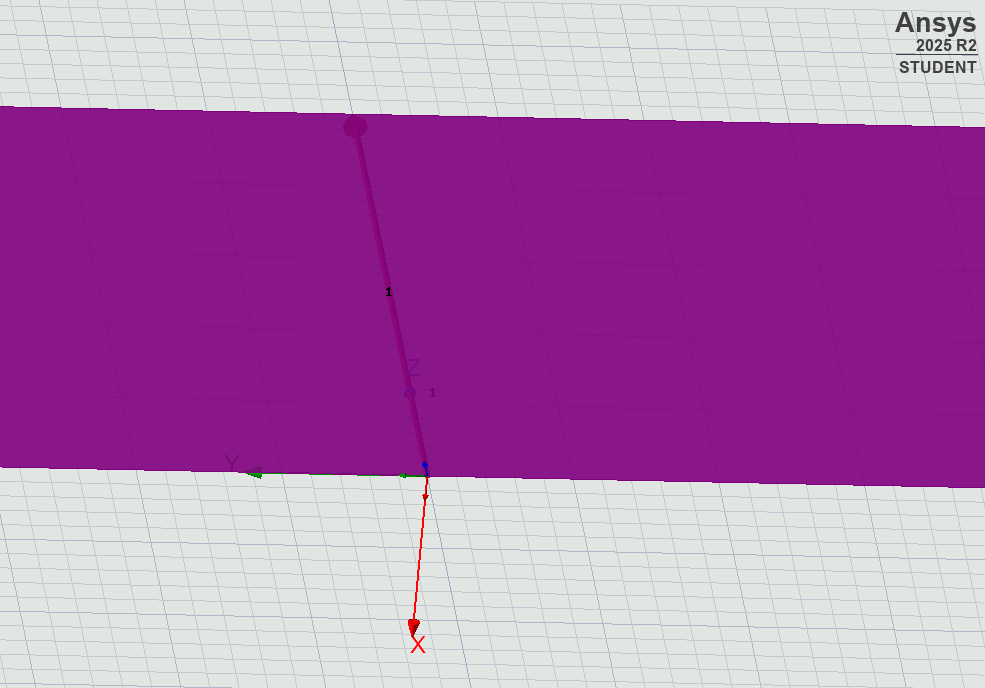
\includegraphics[width=0.7\textwidth]{p13_1.png}
       \caption{端口激励设置完成}
  \end{figure}
\end{enumerate}

\subsubsection{设置辐射边界条件}

\begin{enumerate}
    \item 在菜单栏中选择 \keyblue{Create Region}，并在弹出的窗口中将 Padding Type 改为 \keyblue{Absolute Offset}，Value 改为 lambda / 4。%，如下图所示：
    
   \begin{figure}[H]
       \centering
       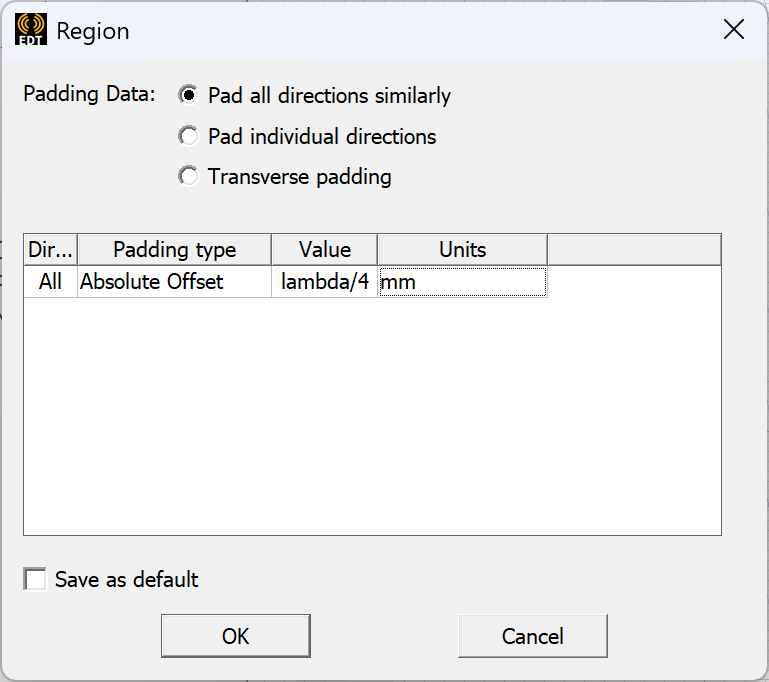
\includegraphics[width=0.5\textwidth]{p15.png}
       \caption{创建辐射边界区域}
       \label{fig:region}
   \end{figure}
    
    \item 双击操作历史树下 Region，打开属性对话框，设置材质为 \keyblue{air}，透明度为 0.8；
    
    \begin{figure}[H]
       \centering
       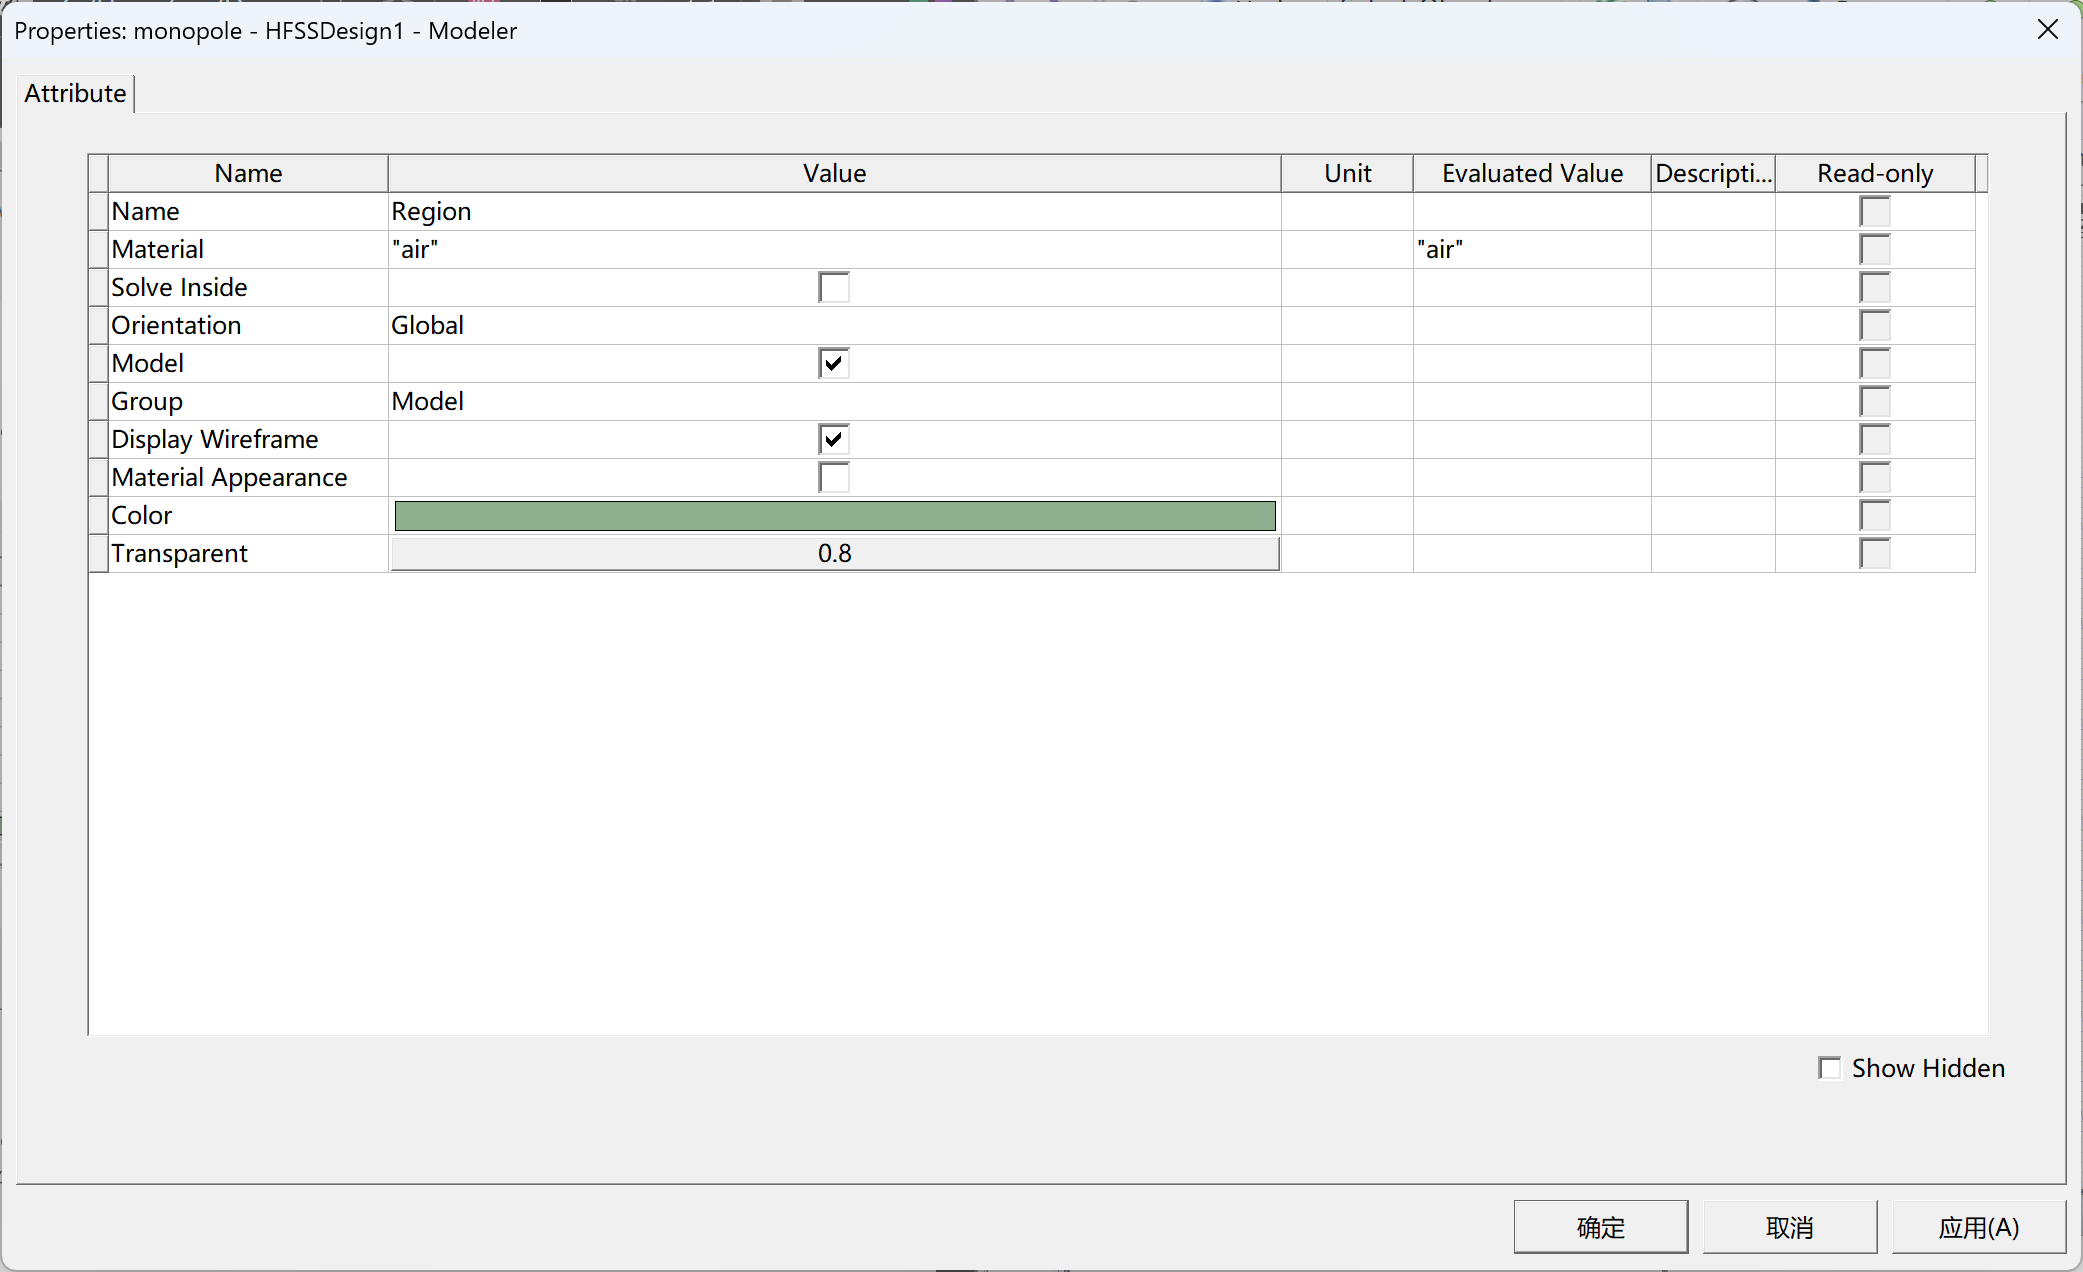
\includegraphics[width=0.5\textwidth]{p16.png}
       \caption{Region设置}
       \label{fig:region}
   \end{figure}

    \item 在操作历史树下单击 \keyblue{Region} 节点，在弹出的快捷菜单中选择 \keyblue{Assign Boundary}-\keyblue{Radiation}，打开辐射边界条件设置对话框，保留默认设置，从而将 Region 表面设置 为辐射边界条件。
    
    至此，单极子天线模型建立完毕。%，完整模型图如下所示：
    
   \begin{figure}[H]
       \centering
       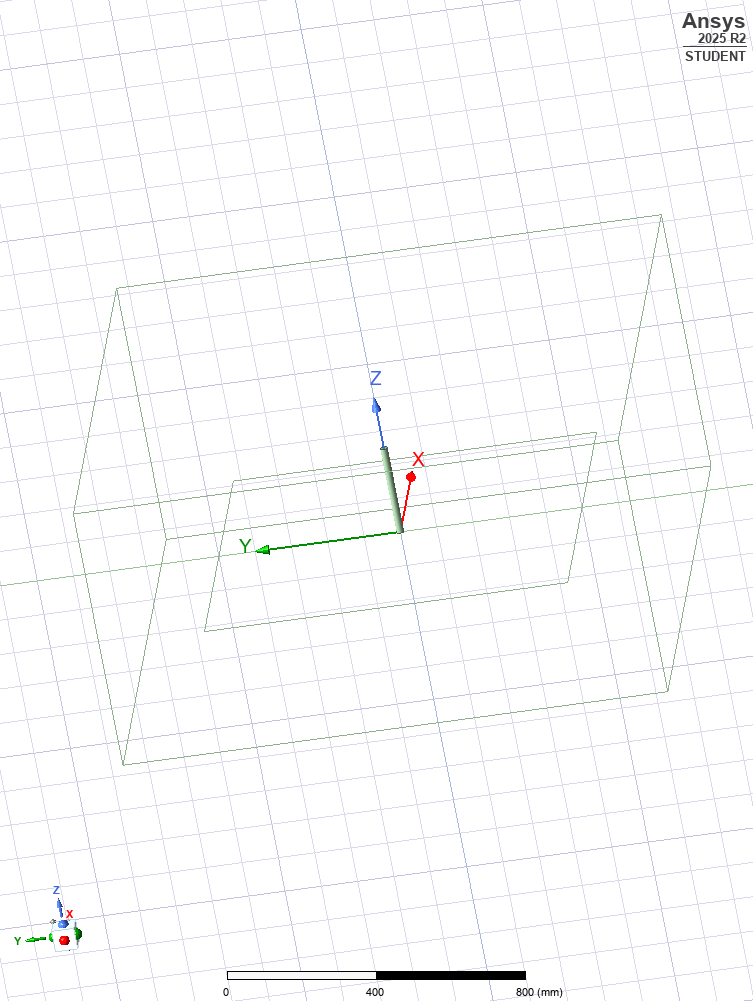
\includegraphics[width=0.5\textwidth]{p17.png}
       \caption{完整的单极天线模型}
       \label{fig:complete_model}
   \end{figure}
\end{enumerate}

\subsection{求解设置}

\begin{enumerate}
    \item 求解频率和网格剖分设置：右键工程树下的 \keyblue{Analysis}，弹出对话框中选中 \keyblue{Add Solution Setup}，将求解频率设为 \keyblue{300MHz}。自适应网格剖分的最大迭代次数设为 20，收敛误差 \keyblue{0.02}。%，如图所示：
    
   \begin{figure}[H]
       \centering
       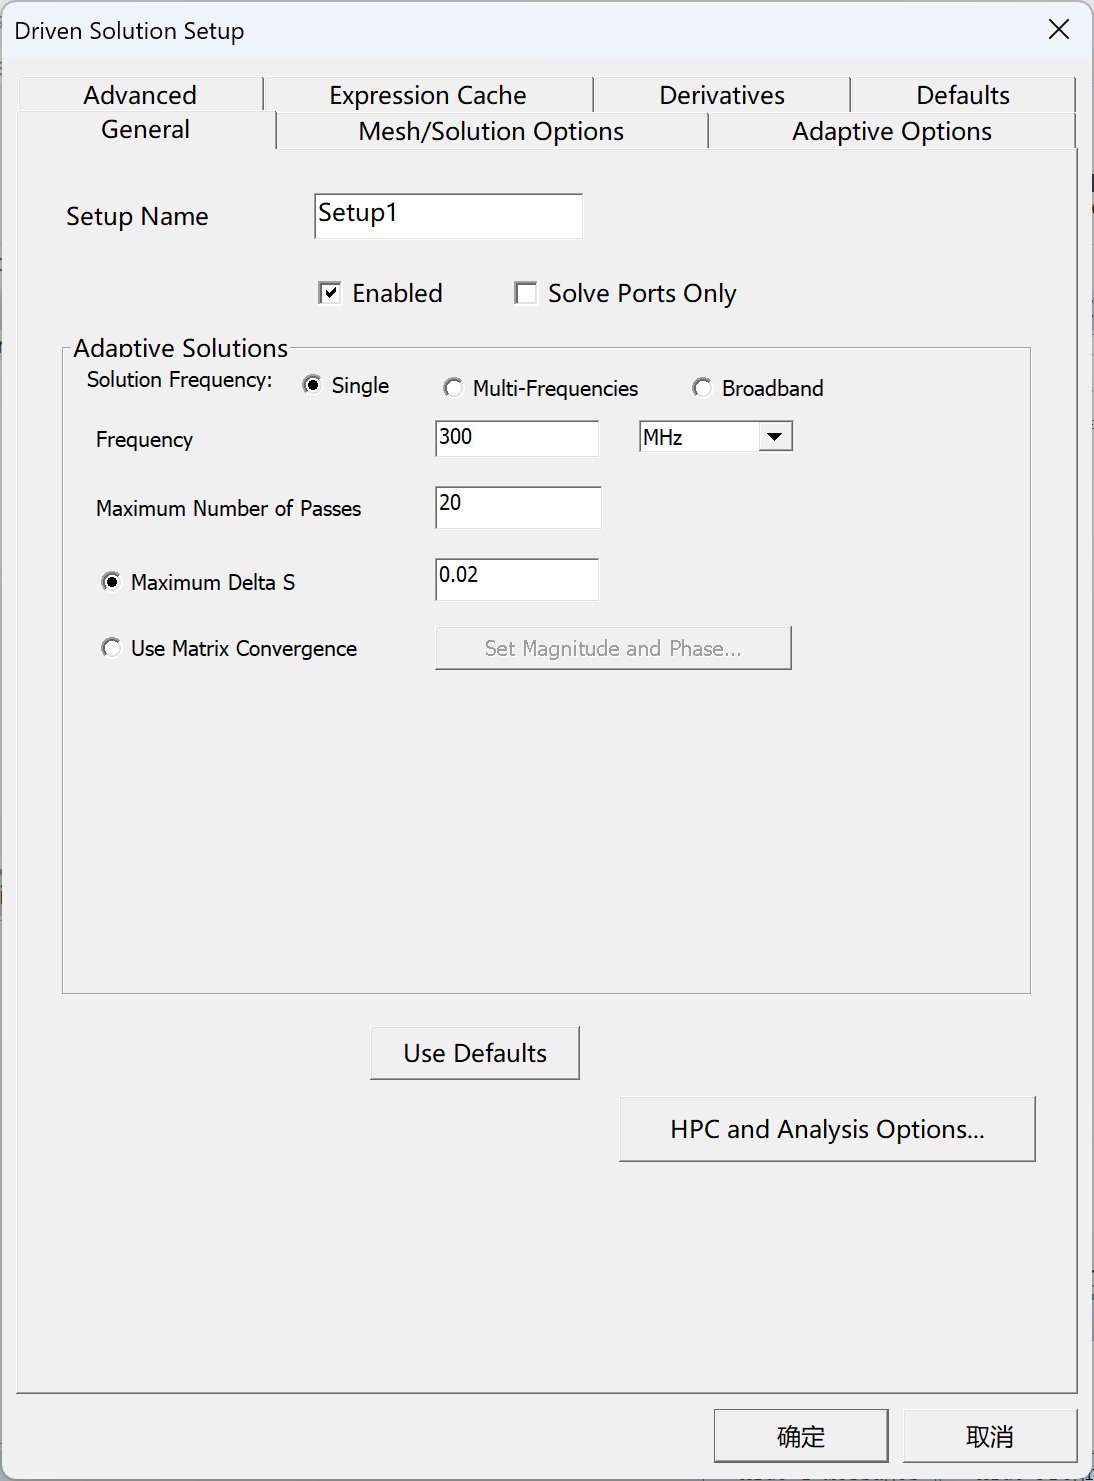
\includegraphics[width=0.5\textwidth]{p19.png}
       \caption{求解设置}
       \label{fig:solution_setup}
   \end{figure}
    
    \item 扫频设置：展开工程树下的 \keyblue{Analysis} 节点，右键单击求解设置项 \keyblue{Setup1}，在弹出的对话框中选择 \keyblue{Add Frequency Sweep}，扫频类型为快速扫频，扫频范围 $200MHz - 400MHz$，点数为 \keyblue{200}。%：
    
   \begin{figure}[H]
       \centering
       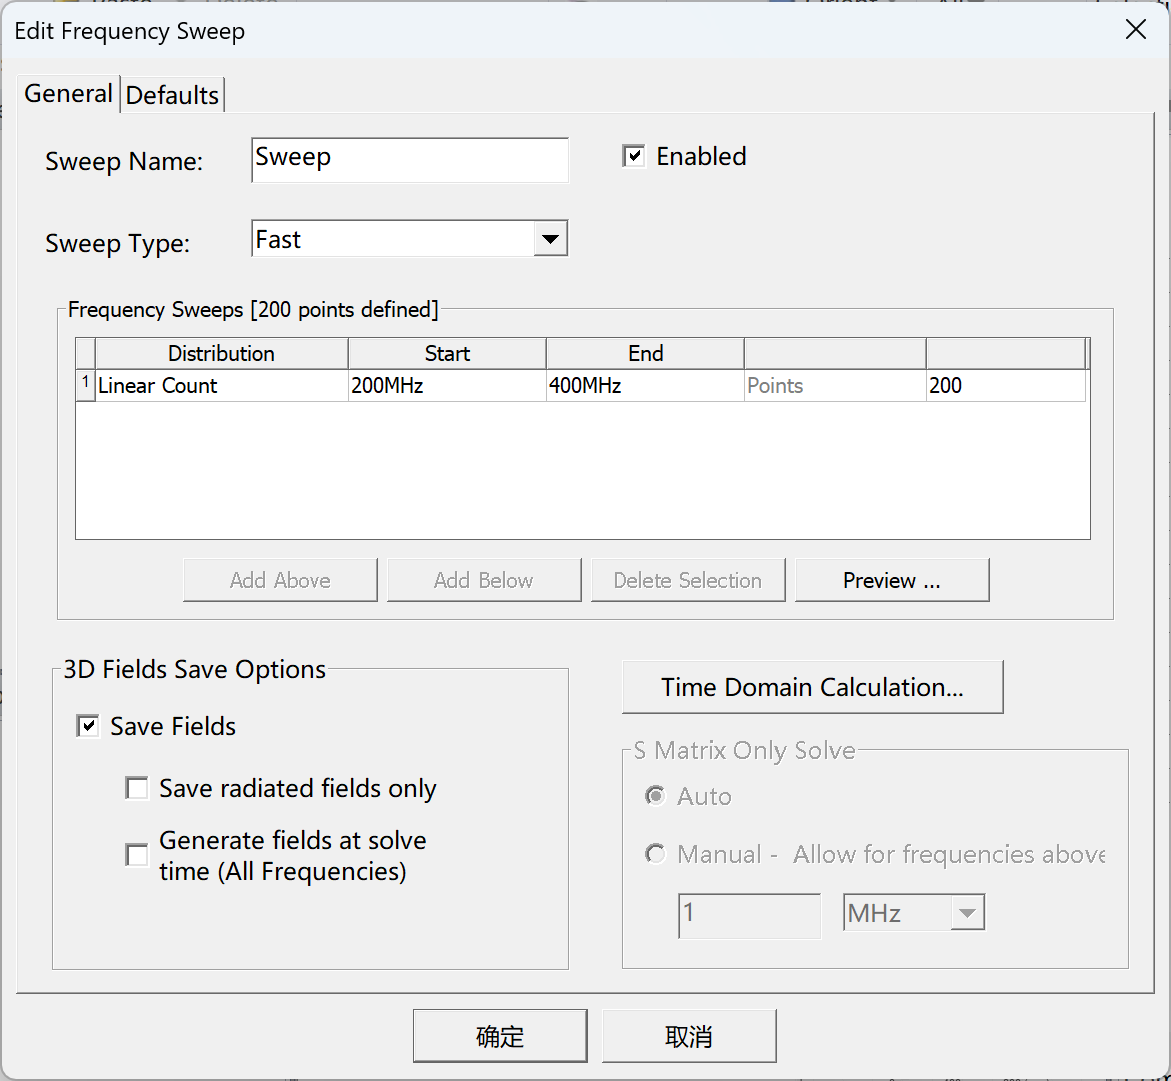
\includegraphics[width=0.5\textwidth]{p20.png}
       \caption{频率扫描设置}
       \label{fig:frequency_sweep}
   \end{figure}
\end{enumerate}

\subsection{设计检查及运行}

\begin{enumerate}
    \item 选择主菜单中 \keyblue{HFSS}-\keyblue{Validation Check}，得到如下对话框，表明设计正确。%：
    
   \begin{figure}[H]
       \centering
       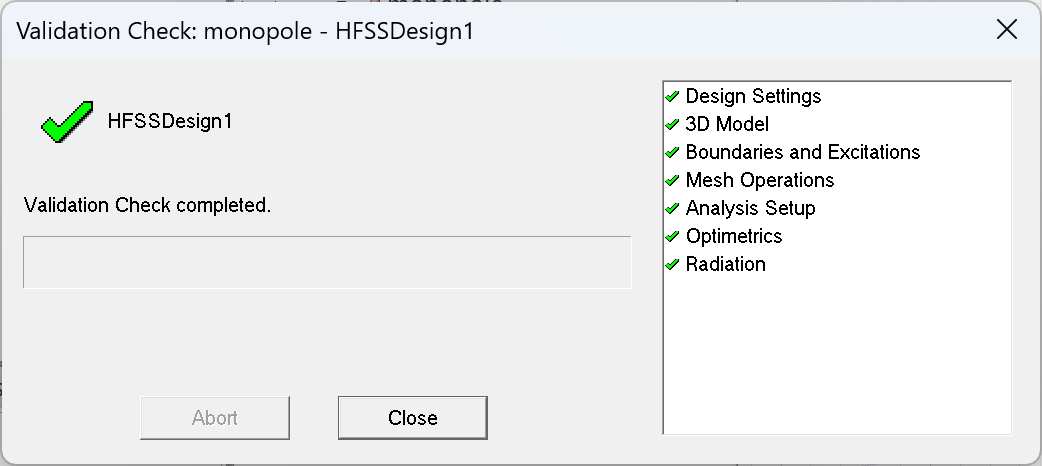
\includegraphics[width=0.6\textwidth]{p21.png}
       \caption{验证检查结果}
       \label{fig:validation}
   \end{figure}
    
    \item 右键单击工程树下的 \keyblue{Analysis}-\keyblue{Setup1}，在弹出菜单中选择 \keyblue{Analyze}，运行分析。
\end{enumerate}

\section{仿真结果与分析}

仿真分析完成后，在数据后处理部分能够给出天线的各项性能参数的仿真分析结果。

\subsection{输入阻抗}

右键单击工程树下的 \keyblue{Results} 节点，在弹出的菜单中选择 \keyblue{Create Model Solution Data Report}-\keyblue{Rectangle Plot} 命令，打开报告设置对话框。%，如图所示：

\begin{figure}[H]
   \centering
   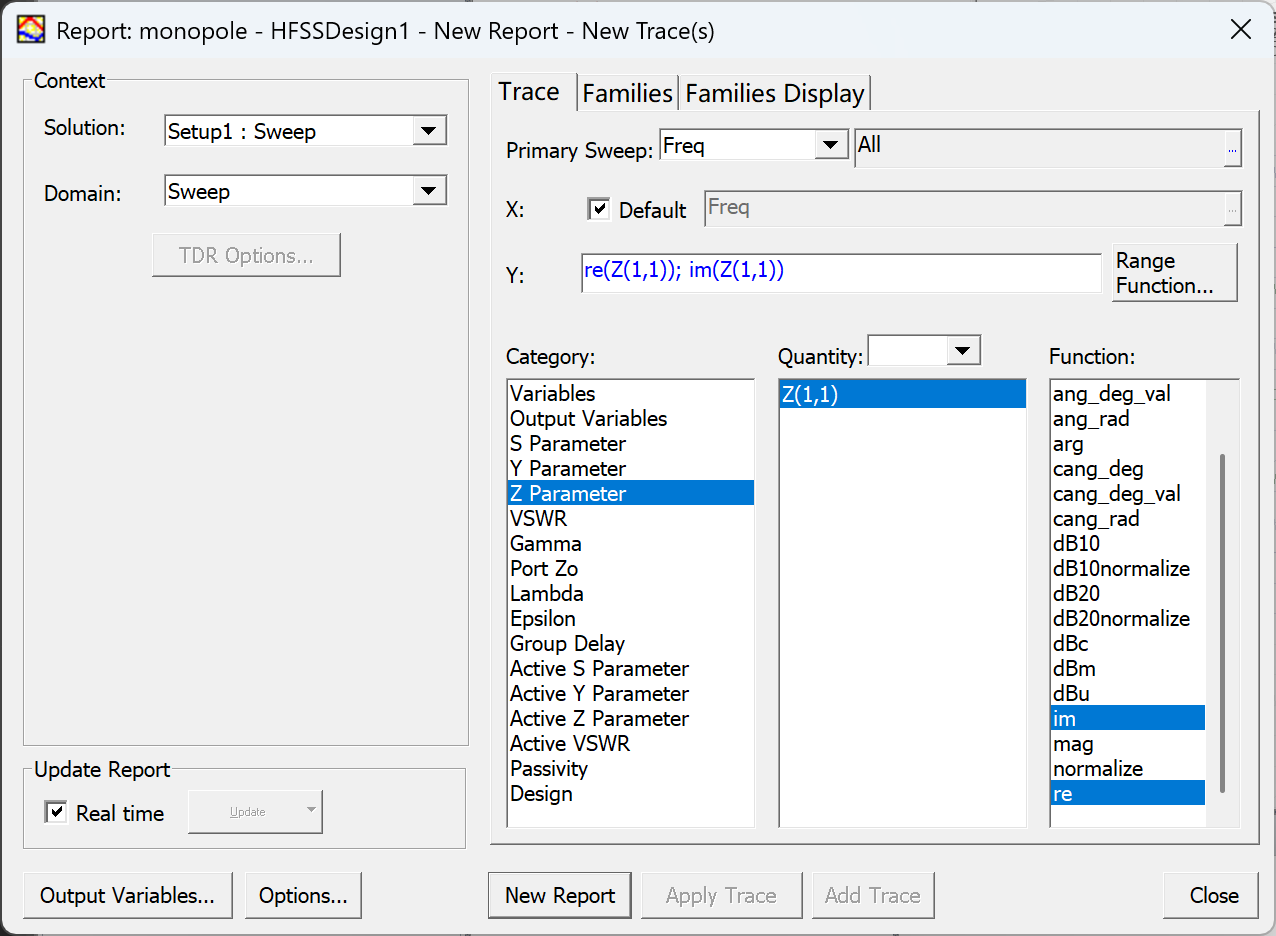
\includegraphics[width=0.85\textwidth]{p23.png}
   \caption{输入阻抗报告设置}
   \label{fig:impedance_report}
\end{figure}

单击 \keyblue{New Report} 按钮，此时可以生成天线输入阻抗分析结果。%：

\begin{figure}[H]
   \centering
   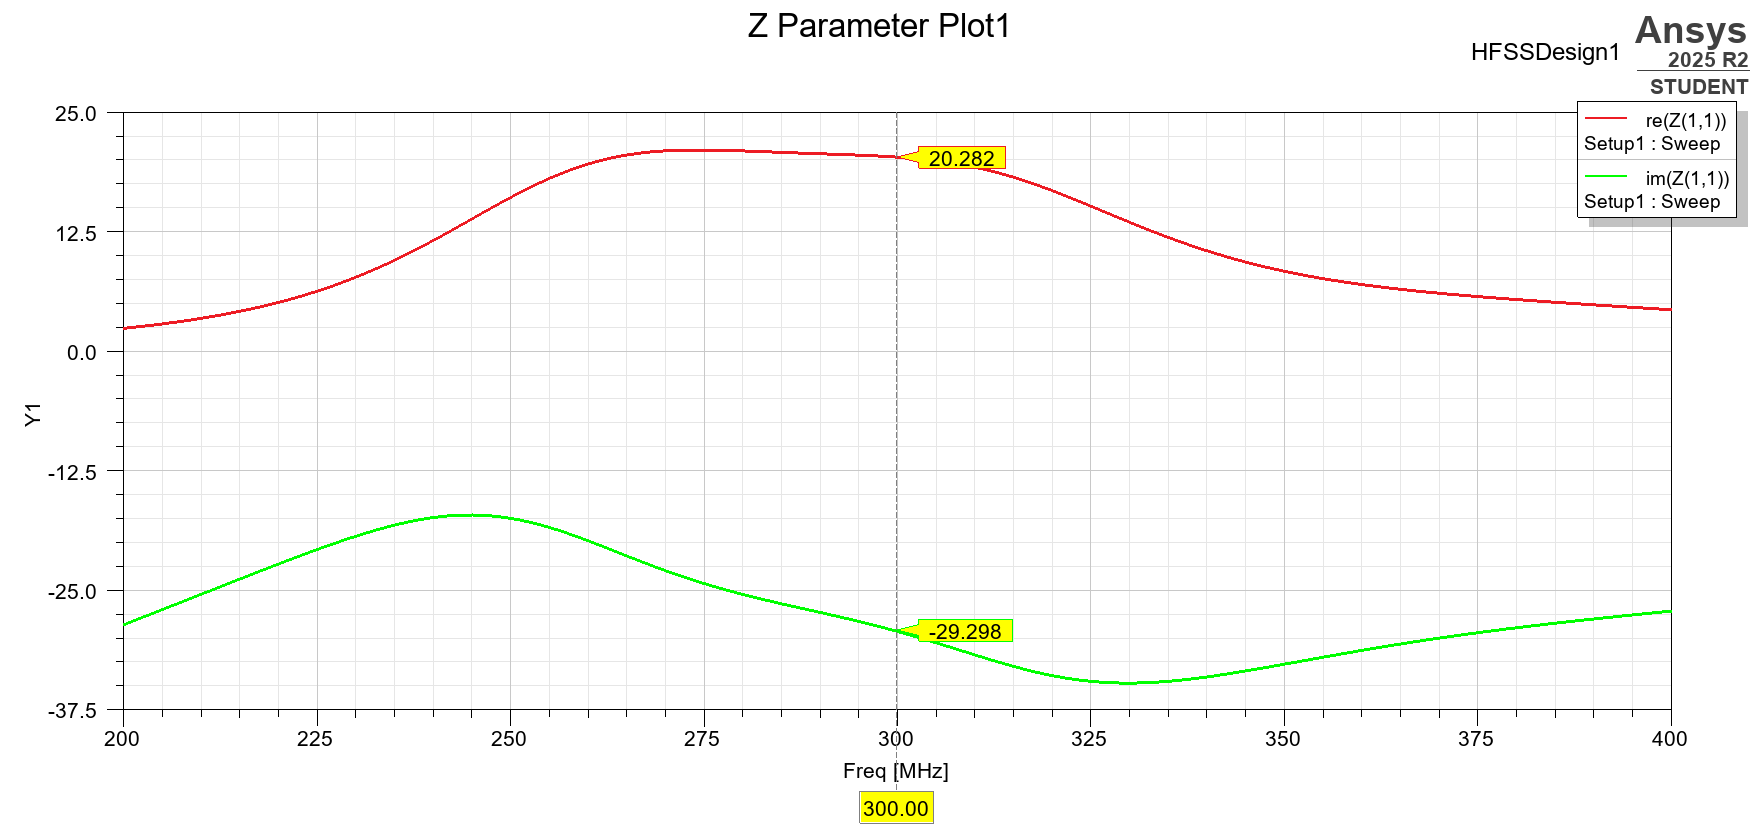
\includegraphics[width=0.85\textwidth]{p24.png}
   \caption{输入阻抗仿真结果}
   \label{fig:impedance_result}
\end{figure}

由仿真结果可知，当连接 $50\Omega$ 传输线时，单极子天线在 300MHz 左右的输入阻抗约为 $(20.282 - j29.298)\Omega$。、
在整个频带内，电抗始终为负，呈容性特征；随频率增加，电阻分量先增大后减小，
电抗的容性分量绝对值呈现先减小后增大再减小的变化趋势，与理论分析相符。

\subsection{电压驻波比}

右键单击工程树下的 \keyblue{Results} 节点，在菜单中选择 \keyblue{Create Model Solution Data Report}-\keyblue{Rectangle Plot} 命令，打开报告设置对话框。%，按下图设置：

\begin{figure}[H]
   \centering
   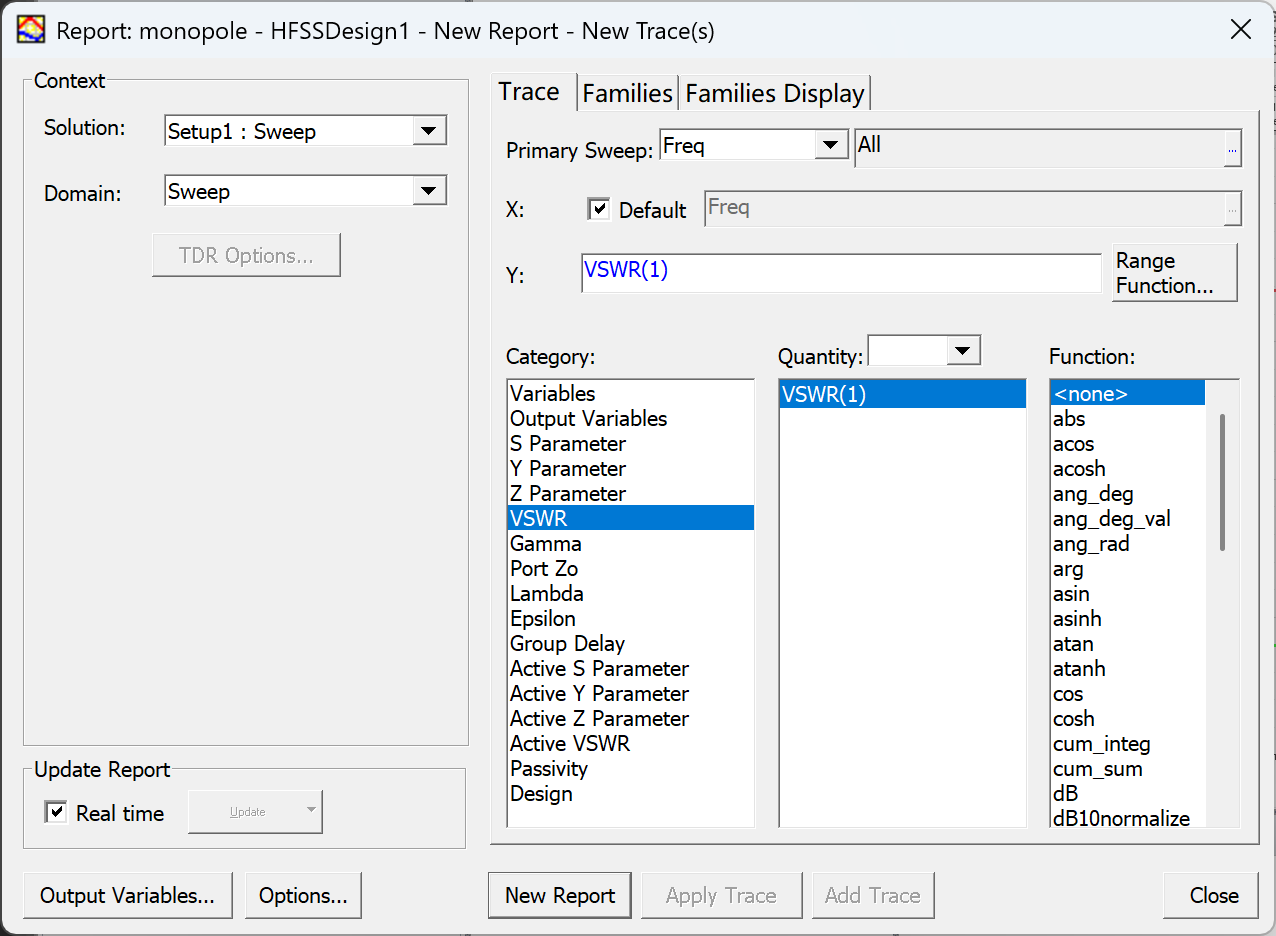
\includegraphics[width=0.9\textwidth]{p25.png}
   \caption{VSWR 报告设置}
   \label{fig:vswr_report}
\end{figure}

单击 \keyblue{New Report}，得到天线的驻波比分析结果。%：

\begin{figure}[H]
   \centering
   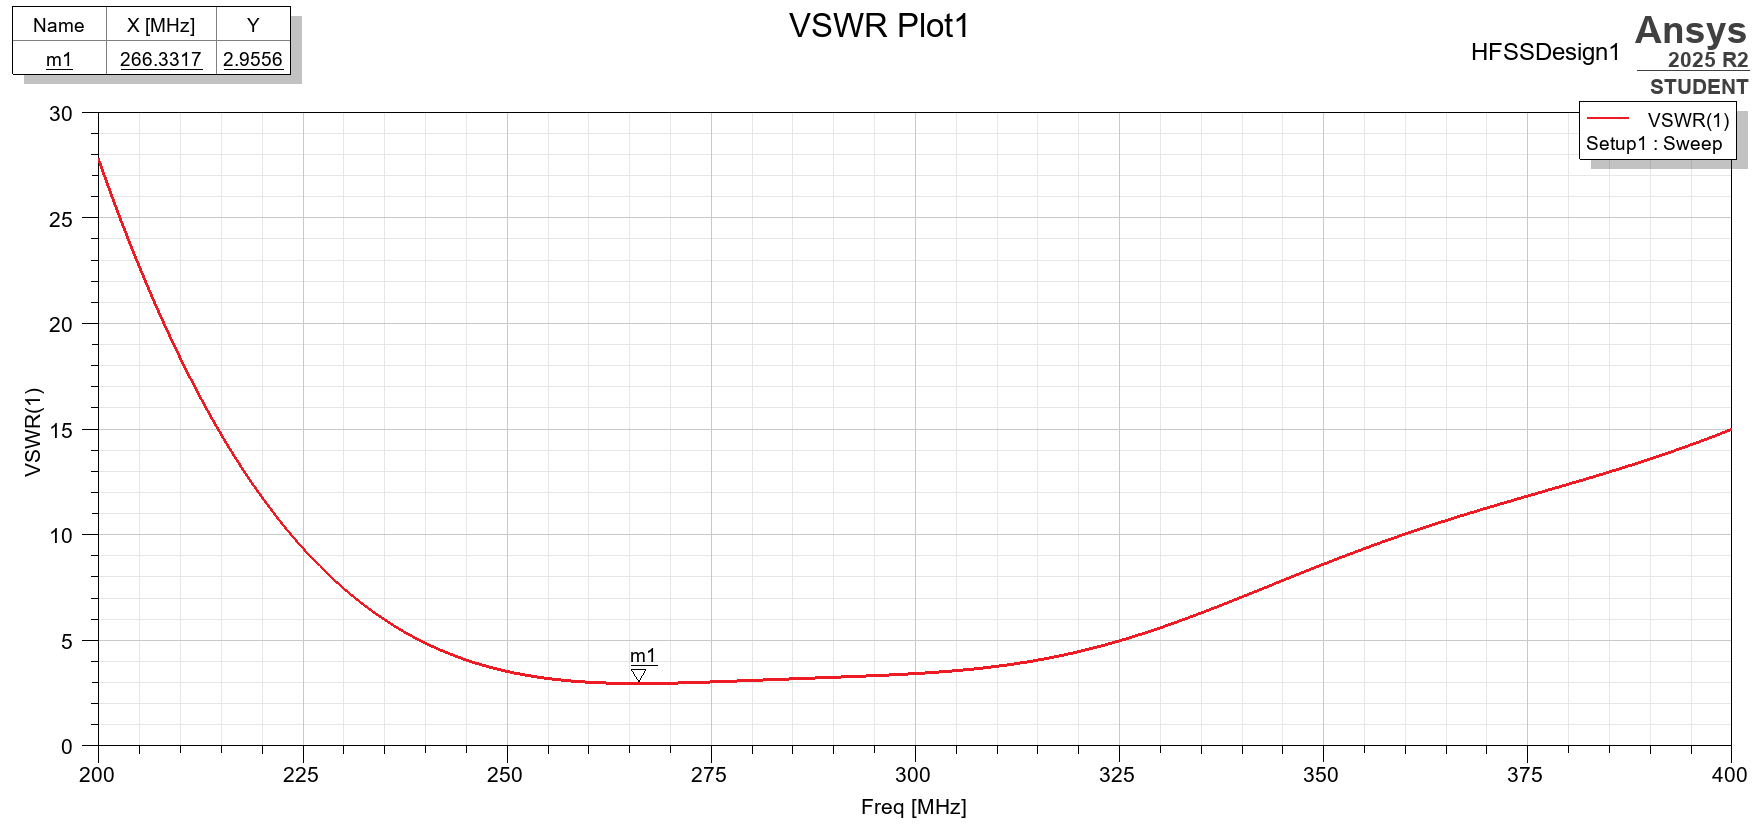
\includegraphics[width=0.9\textwidth]{p26.png}
   \caption{VSWR 仿真结果}
   \label{fig:vswr_result}
\end{figure}

\textbf{结果分析：}由仿真结果可知，当连接 $50\Omega$ 传输线时，单极子天线的电压驻波比 \textit{VSWR} 在 266.3MHz 附近取得最小值，
最小值约为 2.95，此时天线的反射相对较小，有较好的工作性能；在其余频段，天线的电压驻波比相对较大，能量的反射损耗较多，不利于天线的正常工作。

\subsection{辐射特性}

\subsubsection{定义辐射表面}

\begin{enumerate}
    \item 定义辐射表面：右键单击工程树下的 \keyblue{Radiation} 节点，在弹出的快捷菜单中选择 \keyblue{Insert Far Field Setup}-\keyblue{Infinite Sphere}，打开 \keyblue{Far Radiation Sphere Setup}，依次完成以下设置。%：
    
   \begin{figure}[H]
       \centering
       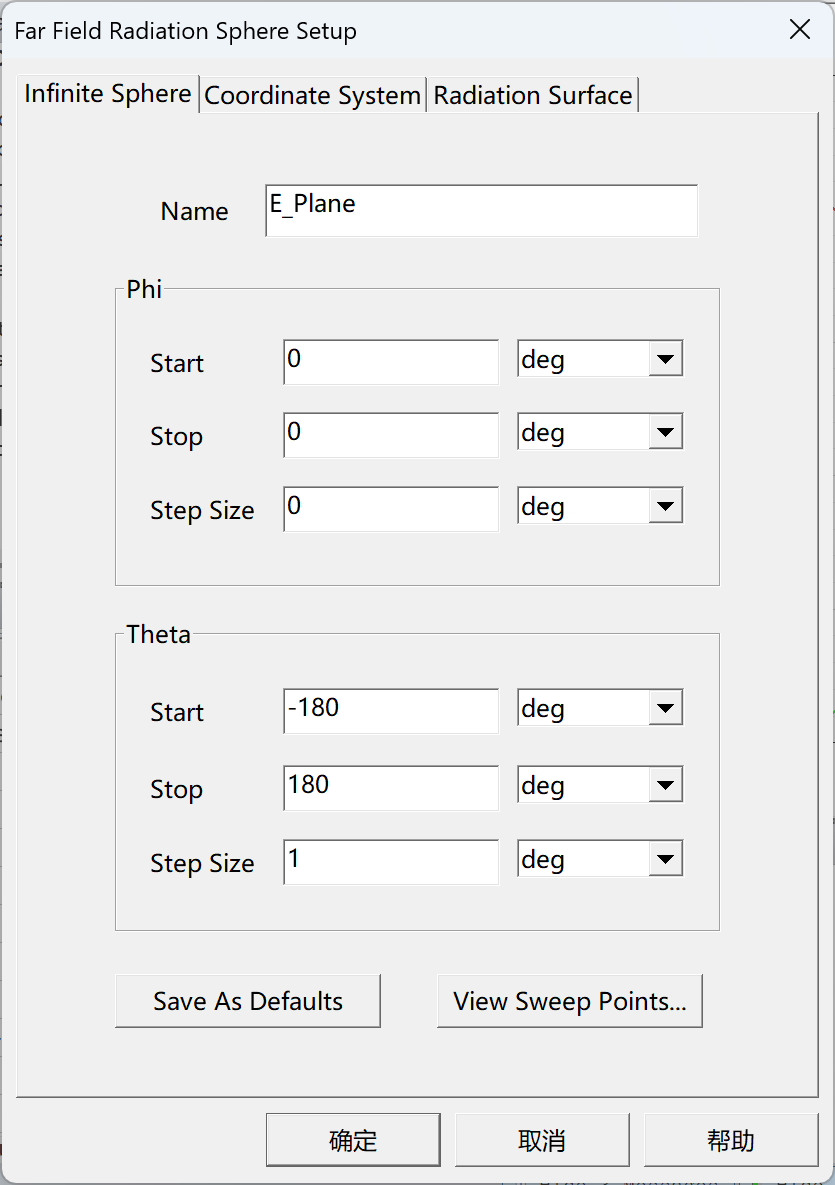
\includegraphics[width=0.32\textwidth]{p27.png}
       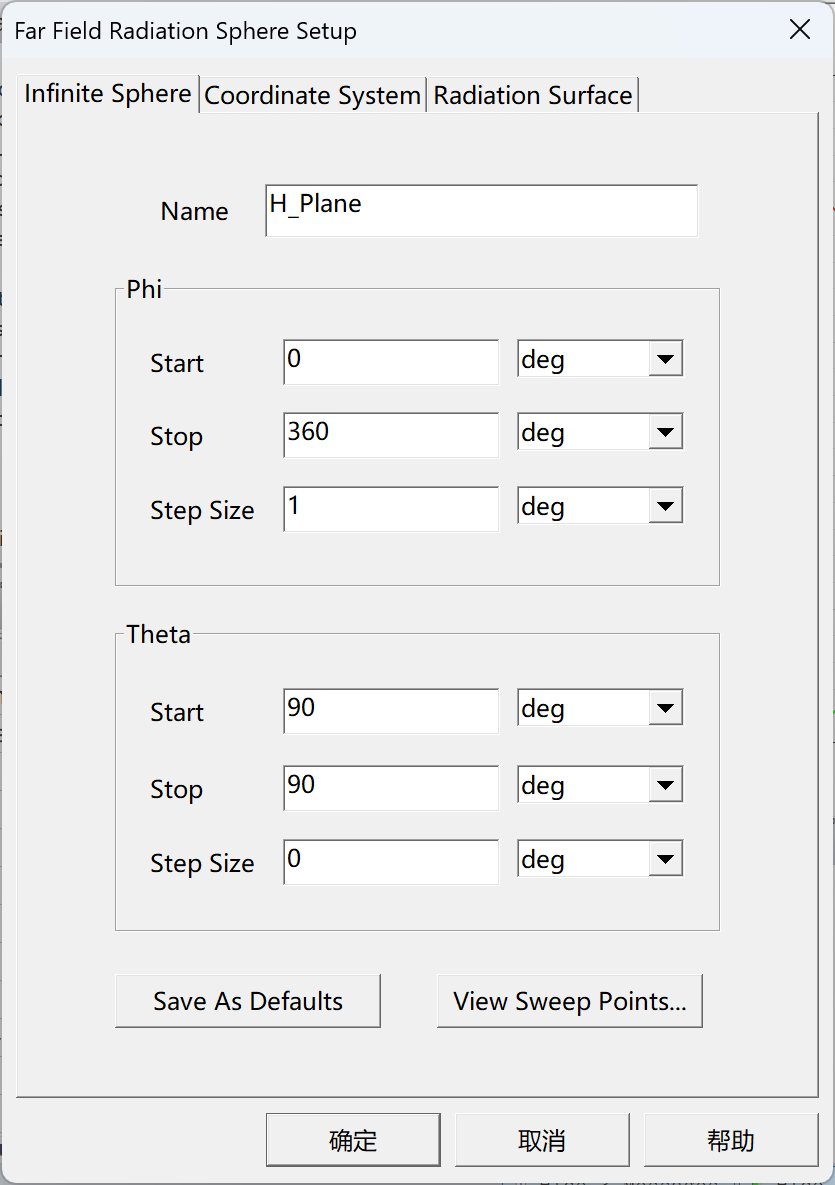
\includegraphics[width=0.32\textwidth]{p28.png}
       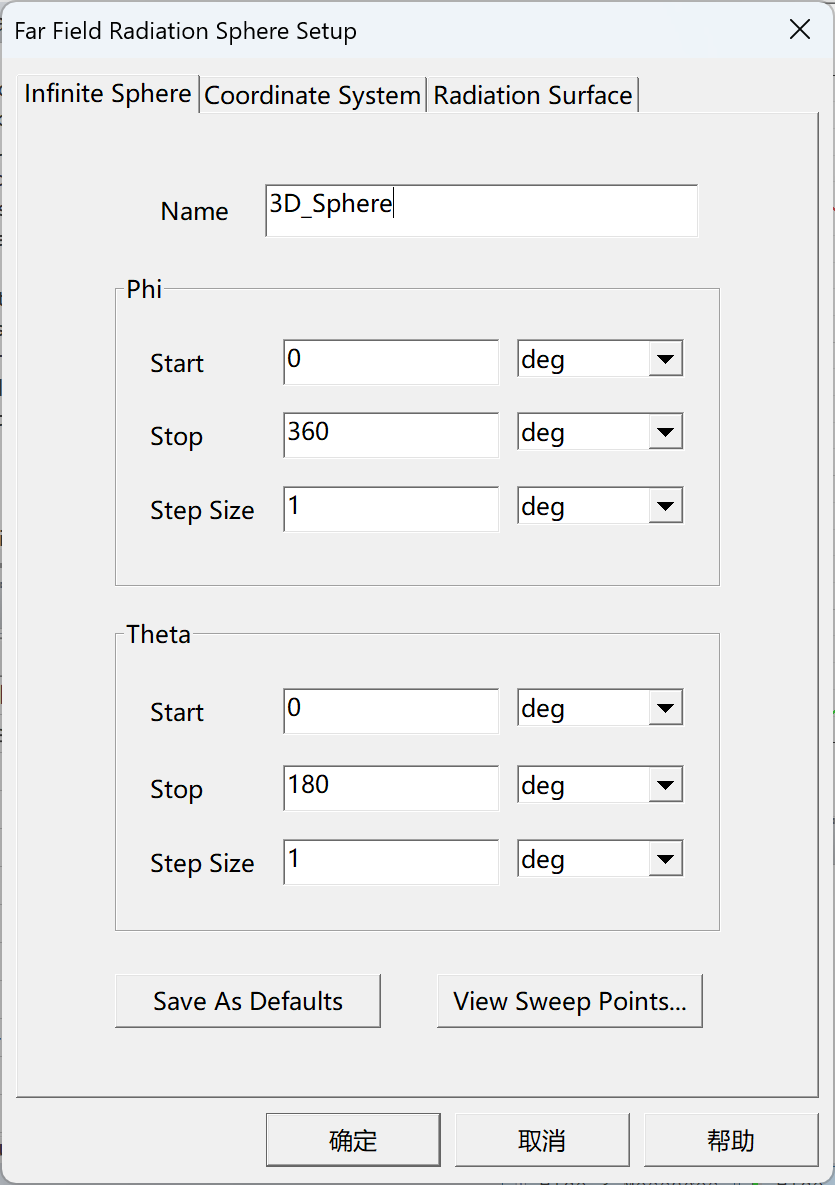
\includegraphics[width=0.32\textwidth]{p29.png}
       \caption{远场辐射球面设置}
       \label{fig:far_field_setup}
   \end{figure}
\end{enumerate}

\subsubsection{xz 面增益方向图 (E 面)}

\begin{enumerate}
    \item 右键单击工程树下的 \keyblue{Results} 节点，在弹出的菜单中选择 \keyblue{Create Far Fields Report}-\keyblue{Radiation Pattern} 命令，如下设置对话框。%：
    
   \begin{figure}[H]
       \centering
       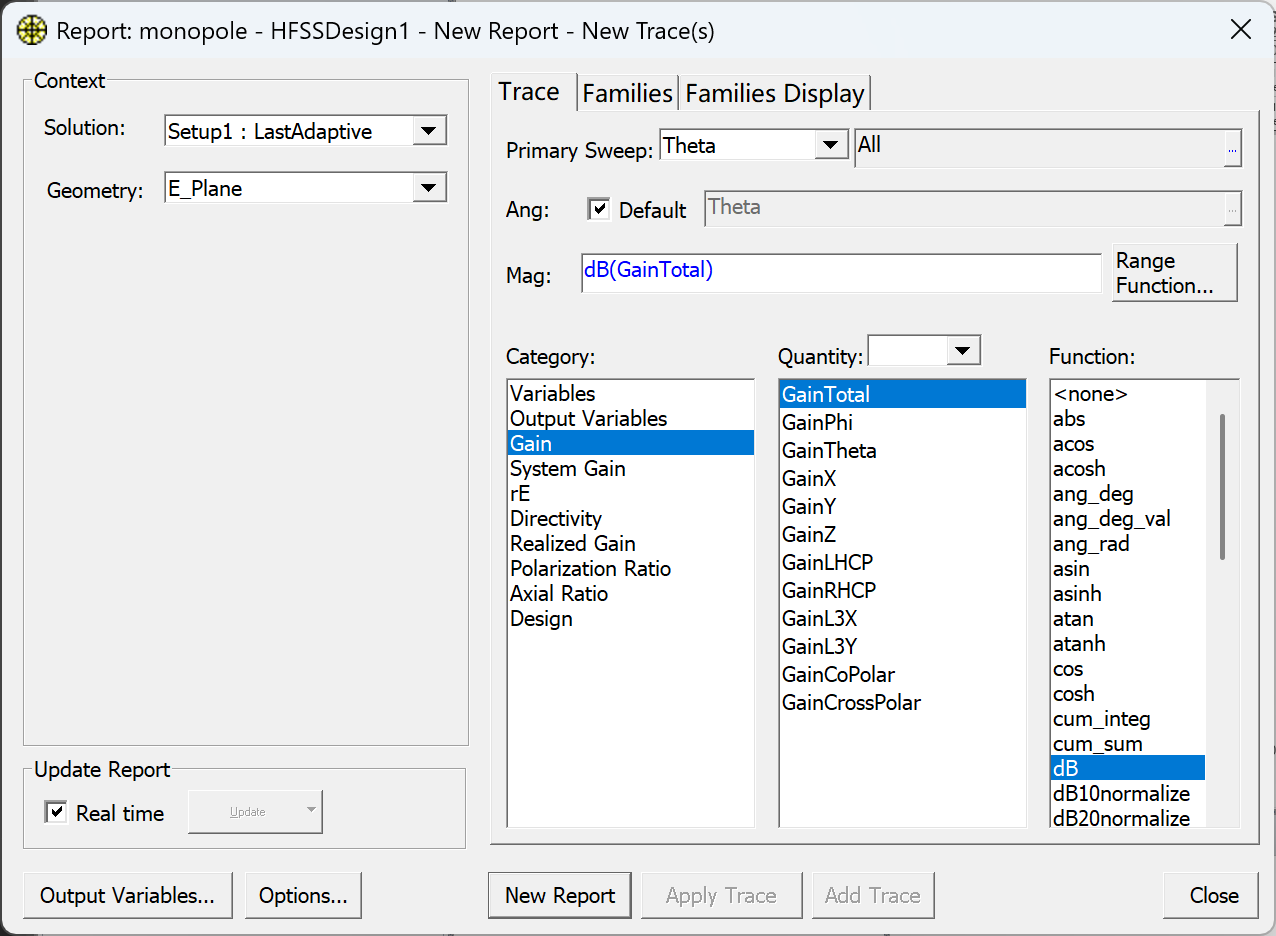
\includegraphics[width=0.85\textwidth]{p30.png}
       \caption{xz 面辐射方向图设置}
       \label{fig:xz_pattern_setup}
   \end{figure}
    
    点击 \keyblue{New Report} 按钮，生成极坐标系下天线的 xz 面增益方向图。%，如图所示：
    
   \begin{figure}[H]
       \centering
       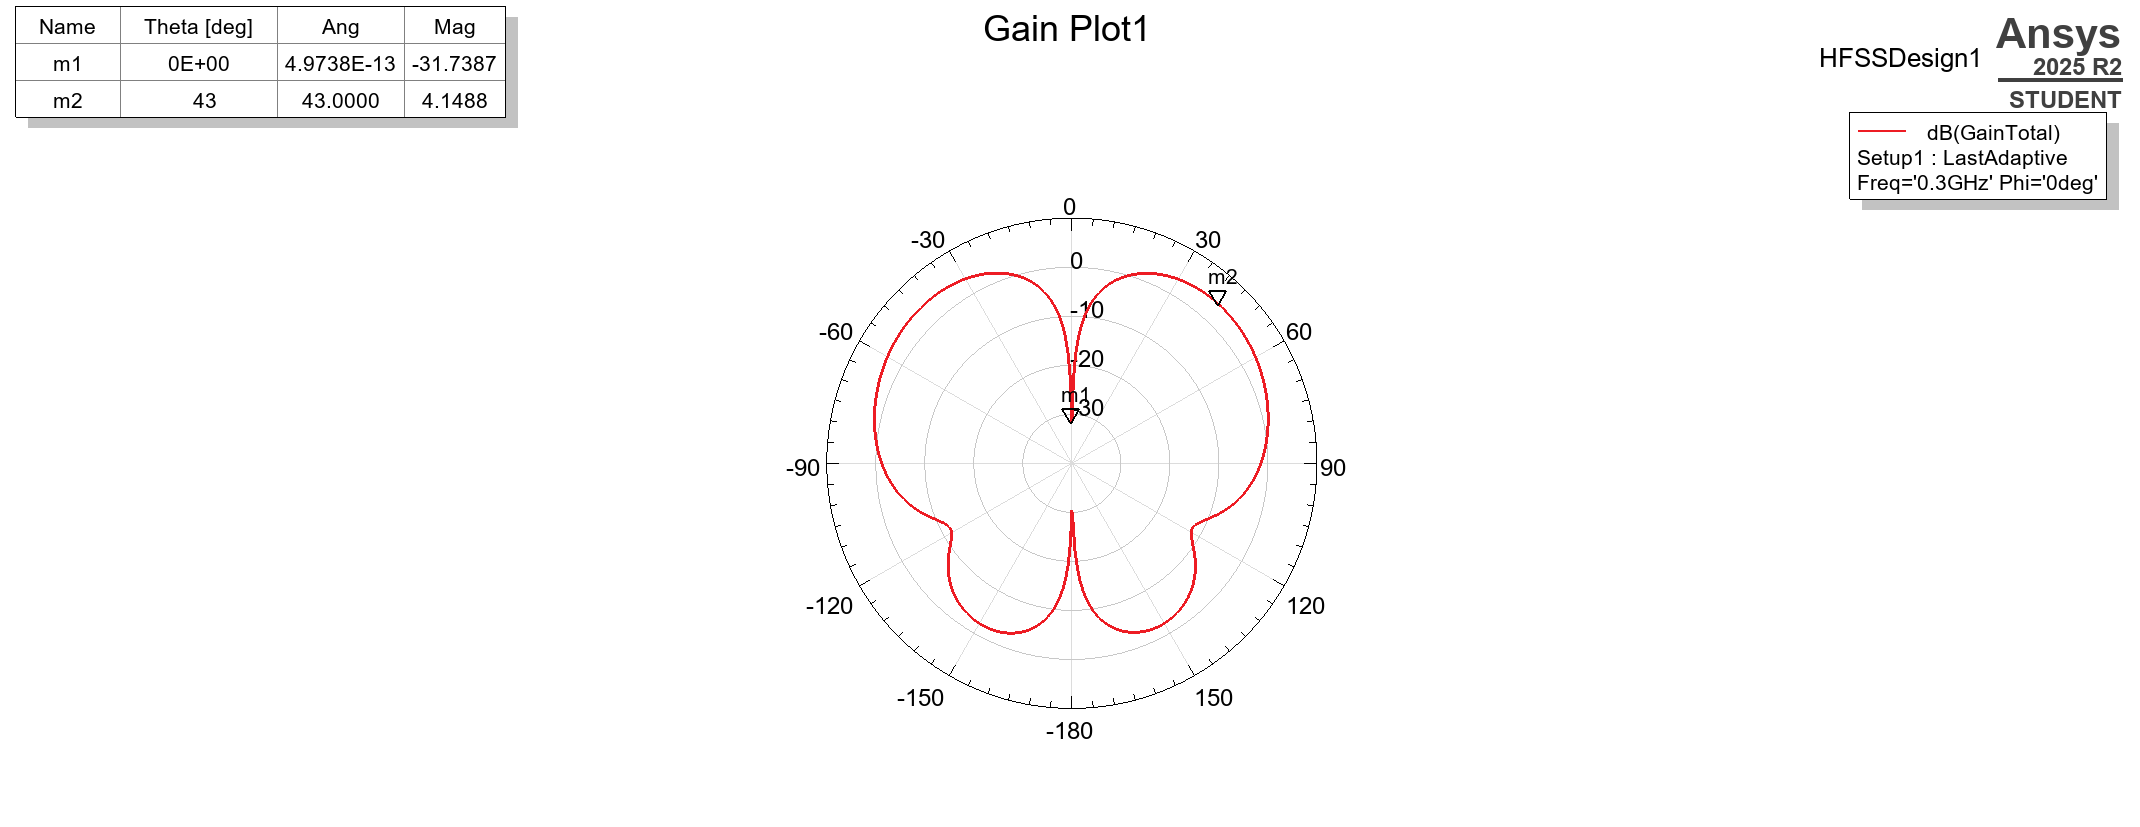
\includegraphics[width=1.0\textwidth]{p31.png}
       \caption{xz 面增益方向图}
       \label{fig:xz_pattern}
   \end{figure}
\end{enumerate}

xz 面（E 面）的增益方向图显示，天线的主瓣最大辐射方向并不在理论上的地平面（$\theta=90^\circ$），而是被抬起到了 $\theta=43^\circ$ 的方向，此时增益最大，约为 4.15 dB。在天顶方向（$\theta=0^\circ$）存在一个明显的零点。此外，由于地平面尺寸有限，在下半空间（$\theta > 90^\circ$）出现了明显的后瓣，这与 1.3 节中关于有限地平面效应的理论分析一致。

\subsubsection{xy 面增益方向图 (H 面)}

\begin{enumerate}
    \item 右键单击工程树下的 \keyblue{Results} 节点，在弹出的菜单中选择 \keyblue{Create Far Fields Report}-\keyblue{Radiation Pattern} 命令，如下设置对话框。%：
    
   \begin{figure}[H]
       \centering
       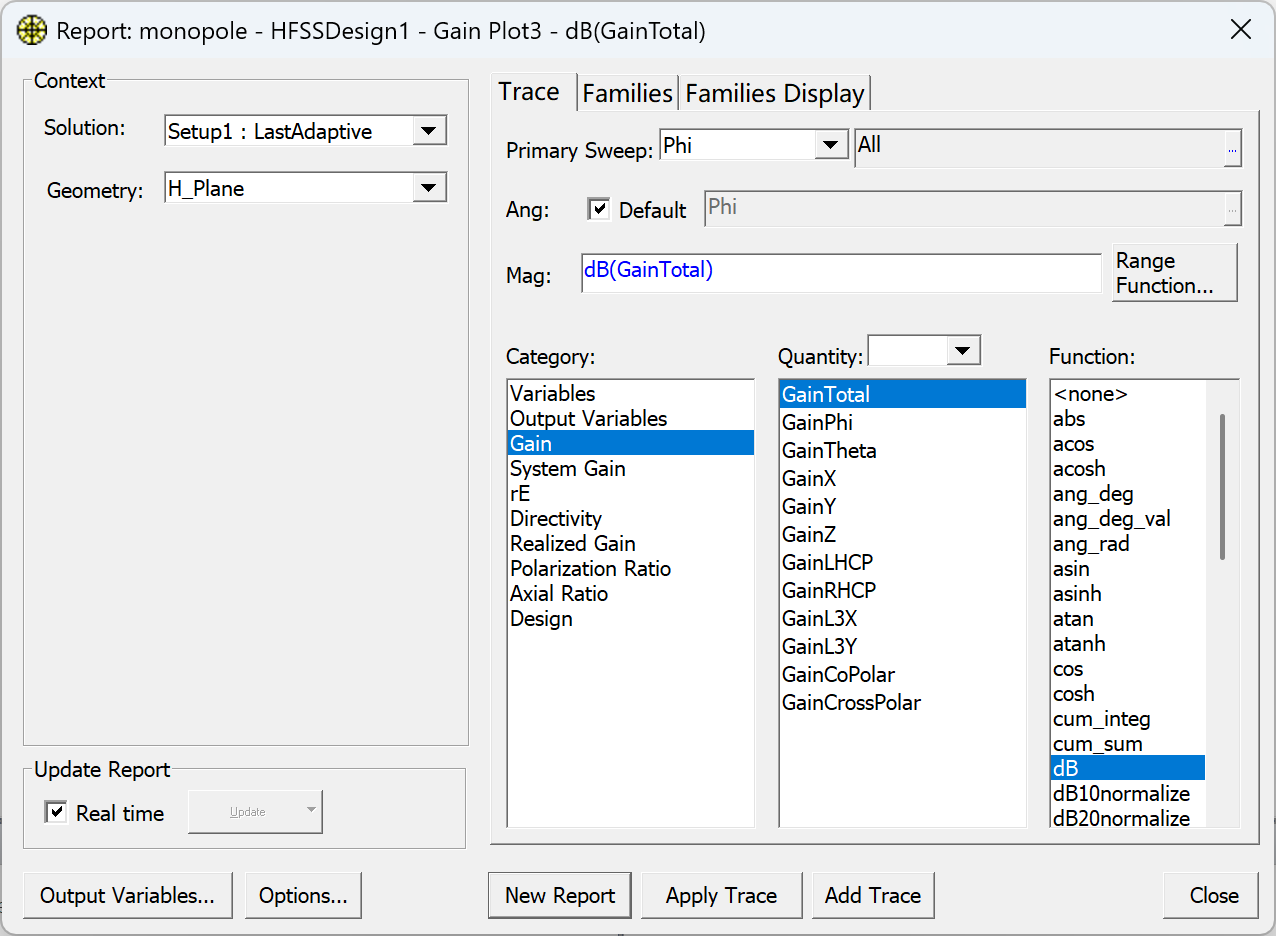
\includegraphics[width=0.85\textwidth]{p32.png}
       \caption{xy 面辐射方向图设置}
       \label{fig:xy_pattern_setup}
   \end{figure}
    
    点击 \keyblue{New Report} 按钮，生成天线的 xy 面增益方向图。%，如图所示：
    
   \begin{figure}[H]
       \centering
       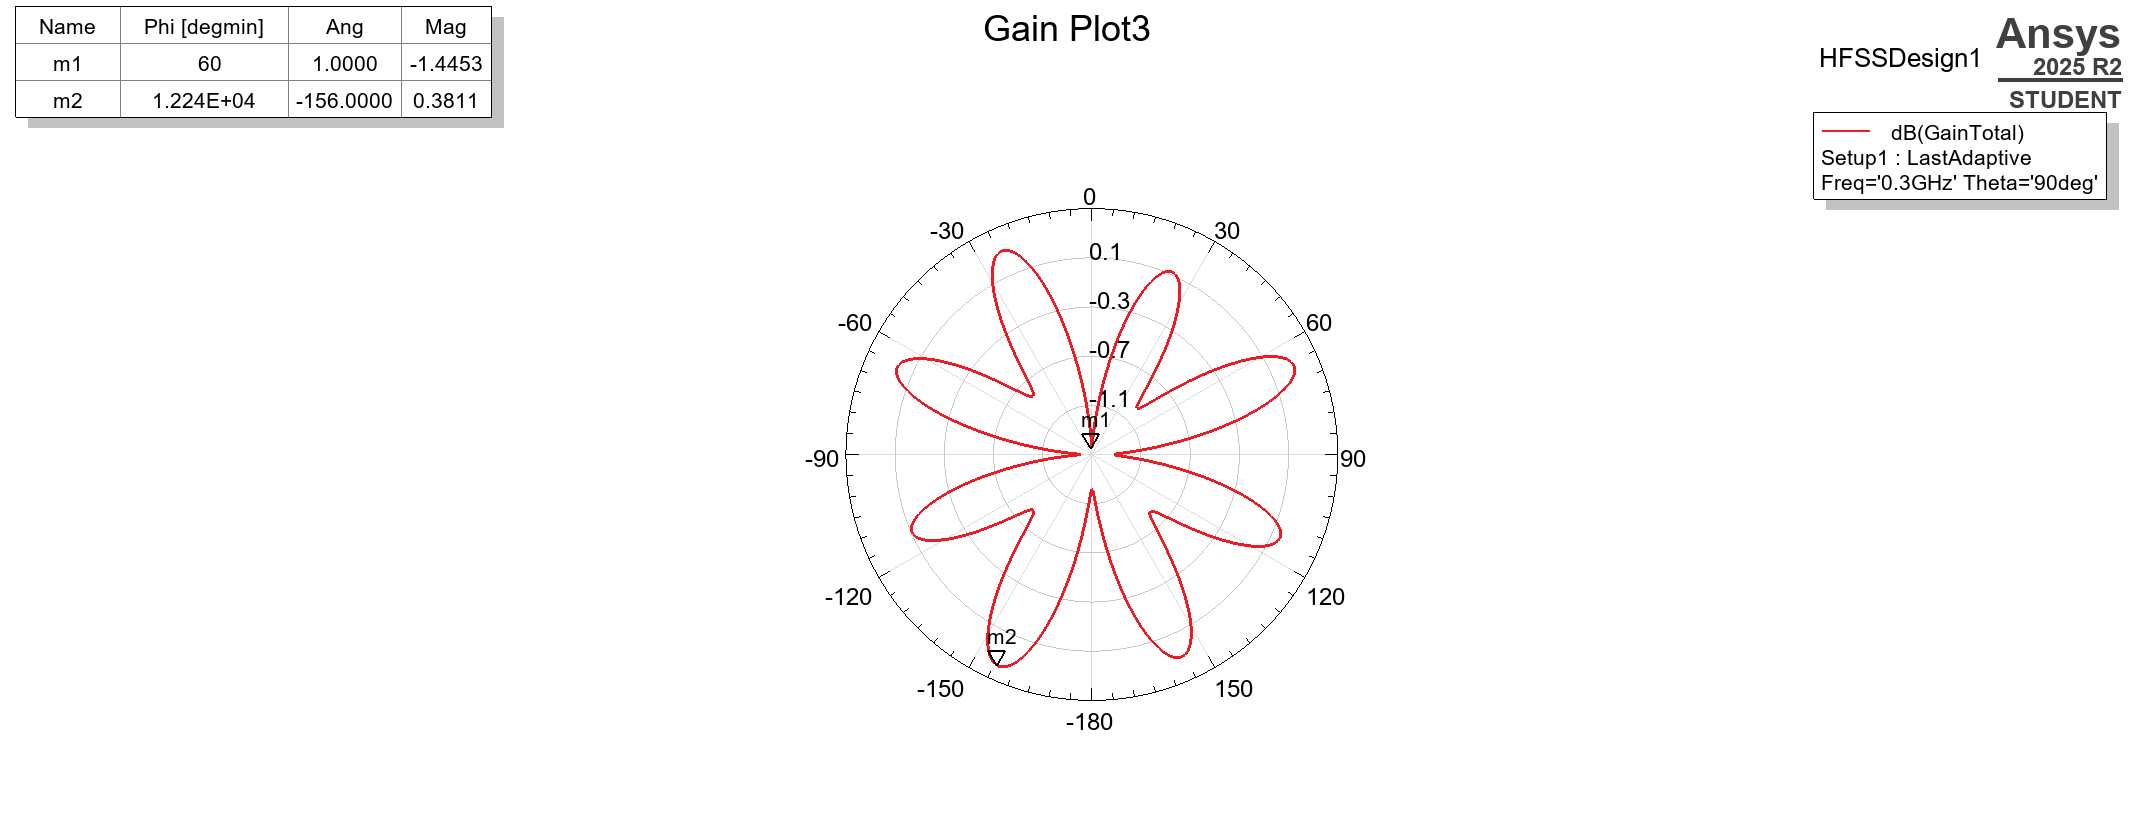
\includegraphics[width=1.0\textwidth]{p33.png}
       \caption{xy 面增益方向图}
       \label{fig:xy_pattern}
   \end{figure}
\end{enumerate}

xy 面（H 面）的增益方向图是在 $\theta=90^\circ$ 的平面上绘制的。与理想单极子天线应呈现全向辐射的理论特性不同，仿真结果显示方向图具有明显的"涟漪"。辐射增益随方位角 $\phi$ 的变化而波动，呈现出多个波瓣，而不是一个平滑的圆形。这是由 1m × 1m 的方形有限地平面边缘发生衍射所引起的。

\subsubsection{三维辐射方向图}

\begin{enumerate}
    \item 右键单击工程树下的 \keyblue{Results} 节点，在弹出的菜单中选择 \keyblue{Create Far Fields Report}-\keyblue{3D Polar Plot} 命令，如下设置对话框。%：
    
   \begin{figure}[H]
       \centering
       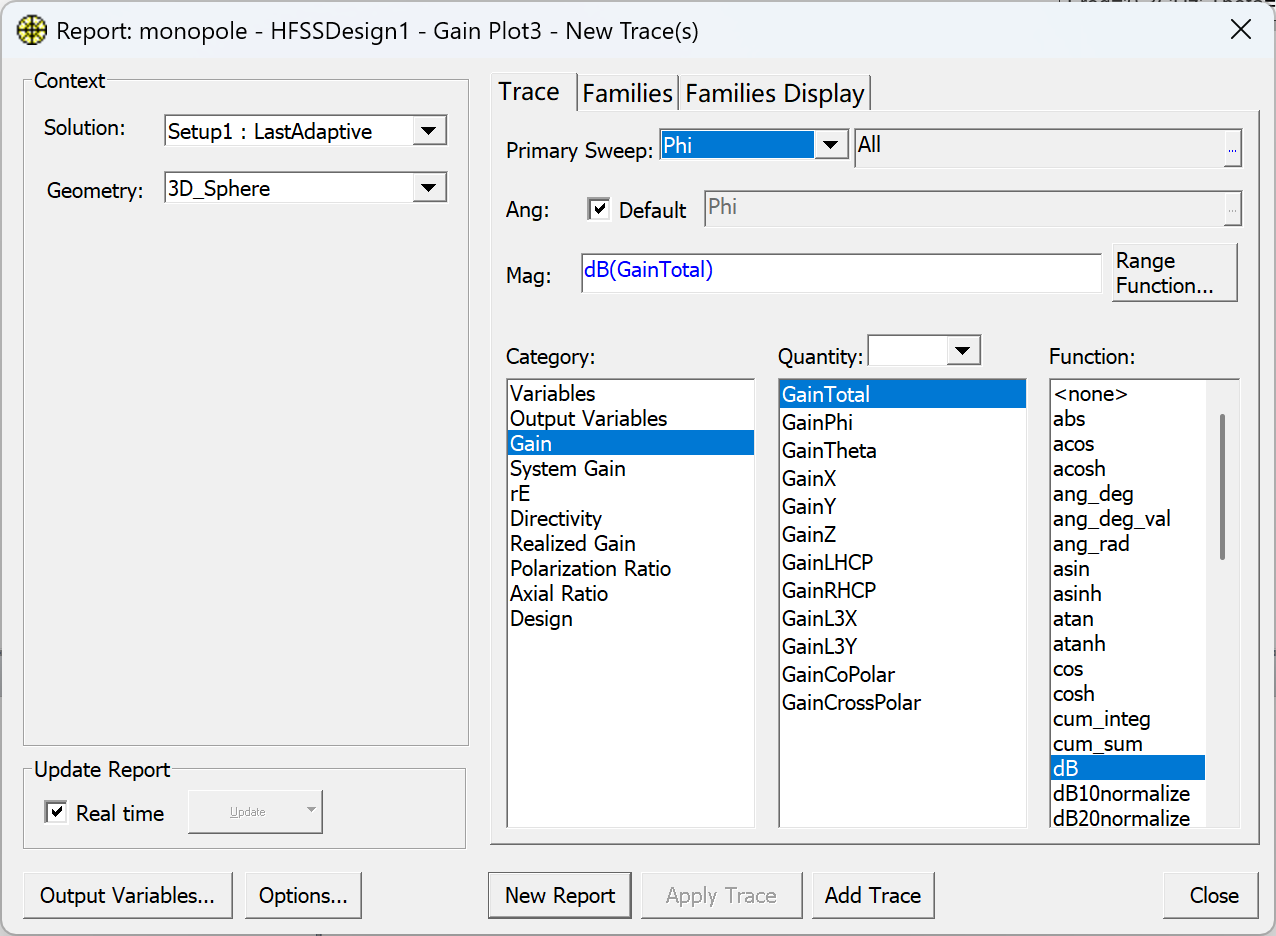
\includegraphics[width=0.85\textwidth]{p34.png}
       \caption{三维极坐标图设置}
       \label{fig:3d_pattern_setup}
   \end{figure}
    
    点击 \keyblue{New Report} 按钮，生成如下结果。%：
    
   \begin{figure}[H]
       \centering
       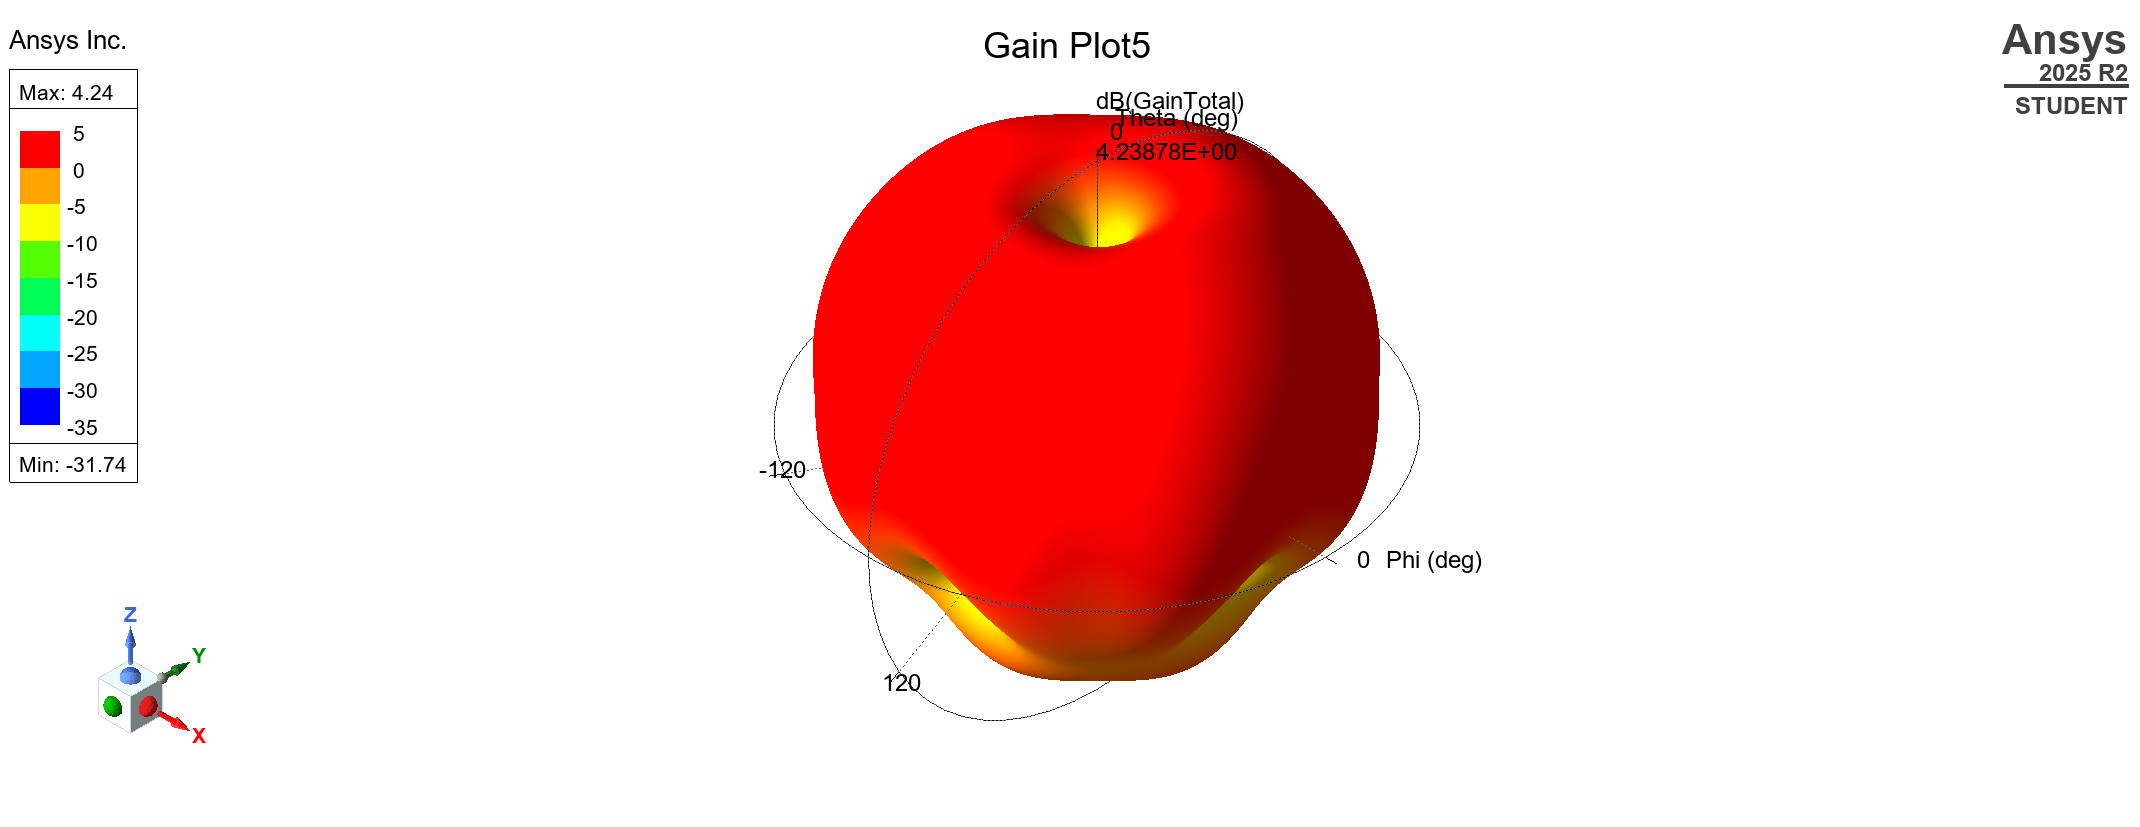
\includegraphics[width=1.0\textwidth]{p35.png}
       \caption{三维辐射方向图}
       \label{fig:3d_pattern}
   \end{figure}
\end{enumerate}

\textbf{实验结论：}三维辐射方向图直观地总结了天线的整体辐射特性。天线的最大增益约为 4.24 dB。仿真结果表明：

\begin{itemize}
    \item \textbf{主瓣上翘：} 天线的主辐射瓣（甜甜圈形状）整体向上倾斜，最大辐射方向并不在水平面上。
    \item \textbf{天顶零点：} 在天线的正上方（天顶）存在一个辐射零点。
    \item \textbf{后瓣泄露：} 由于地平面尺寸有限，天线在下半空间（地平面下方）存在明显的后瓣泄露，能量辐射图样与理想偶极天线的上半空间并不完全相同。
\end{itemize}

这些现象均符合 1.3 节中对有限地平面效应的理论预期。

\section{实验总结与心得体会}

\subsection{实验总结}

本次实验通过 Ansys HFSS 软件，成功仿真了一个中心频率 300MHz 的 $\lambda/4$ 单极子天线。实验的核心目的不仅仅是学习 HFSS 软件操作，更是深入探究了有限尺寸地平面（1m × 1m）对天线性能的实际影响，并将其与基于无限大地平面的经典镜像理论进行了关键对比。通过规范的建模、变量定义、集总端口激励和辐射边界设置，我们获得了天线在 200-400MHz 频带内的输入阻抗、电压驻波比和三维辐射方向图，仿真流程完整且数据详实。

\subsection{心得体会}

本次实验给我最深刻的体会是理想理论与工程现实的显著差距，以及仿真工具在揭示这种差距时不可替代的作用。

\textbf{地平面是天线不可分割的一部分：}经典镜像理论是一个完美的理想模型，它预测 $\lambda/4$ 单极天线的阻抗约为 36.5 $\Omega$。但本次仿真结果显示，在 1m × 1m 的有限地平面上，天线在 300MHz 时的输入阻抗约为 $(20.282 - j19.298)\Omega$，呈现明显的容性，远未达到谐振。这证明了地平面绝非一个被动的"0V 参考面"，而是天线辐射结构的关键组成部分。

\textbf{有限尺寸效应的"代价"：}地平面的有限尺寸（$1\lambda \times 1\lambda$）带来的边缘衍射效应是导致性能偏离的根本原因，具体体现在：

\begin{itemize}
    \item \textbf{谐振点偏移：} 天线的最佳匹配点（VSWR 最小值 $\approx 2.95$）偏移到了 266.3MHz 附近，而非理论上的 300MHz。
    \item \textbf{方向图畸变：} H 面（xy 平面）不再是理想的全向圆形，而是因方形地平面的衍射呈现出明显的波纹。
    \item \textbf{主瓣上翘与后瓣泄露：} E 面（xz 平面）的最大辐射方向从理论的水平方向（$\theta=90^\circ$）被"抬起"到了 $\theta=43^\circ$，最大增益约为 4.24 dB。同时，地平面下方出现了不可忽略的后瓣泄露。
\end{itemize}

通过本次实验，我深刻认识到仿真工具在天线设计中的重要性，以及理论与实践相结合的必要性。有限地平面效应的影响提醒我们，在实际工程应用中必须充分考虑边界条件对天线性能的影响。

\end{document}
